\chapter{Evaluation}%
\label{ch:evaluation}%


In this chapter, we present the evaluation of this thesis.
We choose the joint presentation of the evaluation of all three contributions \C{1}, \C{2}, and \C{3} for increased cohesiveness and clarity.
The evaluation is based on the evaluation scenarios, introduced in \autoref{ch:evaluationscenarios}.

Although all three contributions of this dissertation target confidentiality with regard to uncertainty, they differ in their nature.
For instance, Contribution \C{1} represents a classification, while Contribution \C{3} comprises meta models and analysis approaches.
Thus, we use different evaluation methods such as user studies and the aforementioned evaluation scenarios, which are comparable to case studies.
This matches the findings of \textcite{konersmann_evaluation_2022}, who conducted a \acf{SLR} with 153 papers on the evaluation methods in software architecture research.
For our research object---architecture analysis methods---case studies, motivating examples, and technical experiments represent the most common evaluation methods \cite{konersmann_evaluation_2022}.
In this case, the most commonly investigated properties are effectiveness, functional suitability, and accuracy, which match the presented evaluation.
For most of the evaluation, we focus on the presented analyses, not the presented meta models.
Following the definition of \textcite{stachowiak_allgemeine_1973}, every model has pragmatism, in our case, to serve the analysis.
Thus, evaluating the analysis indirectly also evaluates the underlying models \cite{walter_context-based_2023}.

The evaluation follows a comprehensive \acf{GQM} approach \cite{basili_goal_1994,basili_methodology_1984}.
A \emph{goal} is on the conceptual level and describes a quality to evaluate, i.e., the aforementioned properties to investigate.
An evaluation can have multiple goals.
A \emph{question} is on the operational level and describes how the quality is measured or assessed.
Each goal can have multiple questions.
A \emph{metric} is on the quantitative level and describes the data that is associated with the question.
Each question can have multiple metrics.
A \ac{GQM} plan helps align quality, assessment, and data to minimize the risk of collecting meaningless results \cite{basili_methodology_1984}.
It also helps to structure the evaluation and increases reproducibility.
We number all goals, questions, and metrics and use labels throughout this chapter.

The remainder of this chapter is structured as follows:
We introduce the \ac{GQM} plans for evaluating all contributions \C{1} -- \C{3}.
Then, we present the evaluation design and results for each contribution separately.
We individually discuss the results and threats to validity according to \textcite{runeson_guidelines_2009}.
Last, we give an summary of the evaluation.

\ownpublications{
\fancycite{hahner_architectural_2021}, 
\fancycite{boltz_handling_2022},
\fancycite{walter_architectural_2022},
\fancycite{kaplan_introducing_2022},\linebreak
\fancycite{hahner_model-based_2023}, 
\fancycite{hahner_classification_2023},
\fancycite{hahner_architecture-based_2023},\linebreak
\fancycite{boltz_extensible_2024},
\fancycite{hahner_arcn_2024}
}





\section{Overview}%
\label{sec:evaluation:overview}

We present the individual \ac{GQM} plans of all three contributions.
The first Contribution \C{1} concerns the classification and identification of uncertainty.
We evaluate the structure's suitability, applicability, purpose, and usability.
The second Contribution \C{2} focuses on architecture-based uncertainty impact analysis using uncertainty propagation.
We evaluate the accuracy and effort reduction.
The third Contribution \C{3} comprises four approaches to uncertainty-aware data flow analysis.
We evaluate the accuracy and scalability.

In total, our \ac{GQM} plans comprise 8 goals, 19 questions, and 32 metrics.
In the following, we show the tree of each evaluation goal and then discuss its questions and metrics.


\subsection{Evaluation Plan for the First Contribution}

The first Contribution \C{1} introduces a classification of software-architectural uncertainty regarding confidentiality \cite{hahner_classification_2023}.
Additionally, it includes means to identify uncertainty sources based on an interactive catalog approach \cite{hahner_arcn_2024}.
This approach is tool-supported by \arcen.
The evaluation of this contribution comprises 4 goals, with a total of 12 questions and 16 metrics.
The evaluation is closely aligned to the simultaneously introduced evaluation method for classifications and taxonomies by \textcite{kaplan_introducing_2022}.

\newcommand{\textGi}[0]{Validate the classification \emph{structure's suitability}, whether it permits the appropriate classification of objects under study with the right scope and granularity.}
\newcommand{\textGiQi}[0]{Has the classification an appropriate level of \emph{generality} and granularity?}
\newcommand{\textGiQii}[0]{Is the classification \emph{appropriate}, comprising only necessary classes?}
\newcommand{\textGiQiii}[0]{Is the classification \emph{orthogonal} without overlapping classes?}
\newcommand{\textGiQiMi}[0]{{\emph{laconicity}}(C,\mathcal{R}) = \frac{\sum\nolimits_{R\in \mathcal{R}} \sum\nolimits_{r\in R} \text{laconic}(C,R,r)}{\sum\nolimits_{R\in \mathcal{R}} \lvert R \rvert} \in [0,1]}
\newcommand{\textGiQiMii}[0]{{\emph{lucidity}}(C,\mathcal{R}) = \frac{\sum\nolimits_{c\in C}\,(\min\nolimits_{R\in\mathcal{R}}\,\text{lucid}(C,R,c))}{\lvert C \rvert} \in [0,1]}
\newcommand{\textGiQiiMi}[0]{{\emph{completeness}}(C,\mathcal{R}) = \frac{\sum\nolimits_{R\in \mathcal{R}} \sum\nolimits_{r\in R} \text{complete}(C,R,r)}{\sum\nolimits_{R\in \mathcal{R}} \lvert R\rvert} \in [0,1]}
\newcommand{\textGiQiiMii}[0]{{\emph{soundness}}(C,\mathcal{R}) = \frac{\sum\nolimits_{c\in C}\,(\max\nolimits_{R\in\mathcal{R}}\,\text{sound}(C,R,c))}{\lvert C\rvert} \in [0,1]}
\newcommand{\textGiQiiiMi}[0]{$\emph{orthogonality}(C,\mathcal{R}) \in [0, 1]$, using an orthogonality matrix}
\begin{figure}
    \centering
    \begin{tikzpicture}
      \nodeGtop{1}{\textGi}
      \nodeQtop{1}{1}{\textGiQi}{G1}
      \nodeMtop{1}{1}{1}{$\textGiQiMi$}{Q11}
      \nodeMbottom{1}{1}{2}{$\textGiQiMii$}{M111}
      \nodeQmid{1}{2}{\textGiQii}{M112}
      \nodeMtop{1}{2}{1}{$\textGiQiiMi$}{Q12}
      \nodeMbottom{1}{2}{2}{$\textGiQiiMii$}{M121}
      \nodeQbottom{1}{3}{\textGiQiii}{M122}
      \nodeMonly{1}{3}{1}{\textGiQiiiMi}{Q13}
    \end{tikzpicture}
    \caption{Overview of the \ac*{GQM} plan of the first goal regarding Contribution \C{1}.}
    \label{gqm:plan:g1}
\end{figure}

\paragraph{Goal \goal{1}}\label{gqm:text:g:1}
\autoref{gqm:plan:g1} shows the tree of the first goal.
Following the aforementioned evaluation method \cite{kaplan_introducing_2022}, this goal concerns the classification \emph{structure's suitability}.
This property describes whether a classification is suitable to classify the objects under study.
In our case, the objects under study are sources of uncertainty with respect to confidentiality.
This can be seen as a baseline check as the classification needs to have the right scope and granularity to be suited.
We also motivated the classification in \autoref{ch:classification} with the lack of suitable taxonomies.
We consider three evaluation questions:

\begin{enumerate}[leftmargin=\GQMquestionsIndent]
  \item[\question{1}{1}] \textGiQi 
  \item[\question{1}{2}] \textGiQii
  \item[\question{1}{3}] \textGiQiii
\end{enumerate}

\phantomsection
\label{gqm:text:q:1:1}
The first Question \question{1}{1} asks about the \emph{generality}, where we evaluate the granularity, i.e. if the classification is not too general but also not too specific.
The right level of granularity is important as a classification group objects under study into classes---a too-low number of classes reduces the usefulness of this information, while a high number too-high number of classes introduces noise and makes the classification results hard to understand.
To this end, the evaluation method reuses metrics used to evaluate conceptual models with respect to tools \cite{kaplan_introducing_2022,ananieva_conceptual_2020}.
The \emph{laconicity} (\metric{1}{1}{1}\label{gqm:text:m:1:1:1}) measures the fraction of terms that are uniquely describable.
Given a classification \emph{C}, a finite set of objects under study $\mathcal{R}$, with $R \in \mathcal{R}$ being an object under study with relevant terms $r \in \mathcal{R}$, then $m^C_R \subseteq C \times R$ describes the relation of classes $c \in C$ to relevant terms $r \in R$.
In our classification, we use the term \emph{option} to refer to classes, e.g., \emph{Behavior} uncertainty and \emph{Scenario} uncertainty are two of the 27 options of our classification.
A class is laconic, if there is at most one $c \in C$ with $(c,r) \in m^C_R$.
Based on this, we denote:

\begin{equation*}
  \textGiQiMi
\end{equation*}

\phantomsection
A low laconicity indicates a too fine-grained classification with potentially too many classes to describe the object under study.
Put simply, a concept of an object under study should be only describable using a single class, otherwise the classification structure's suitability could be decreased.
For instance, if we have one object under study, one term that represents \emph{Behavior} uncertainty, and one class to describe it, this class is laconic, thus ${\emph{laconicity}}(C,\mathcal{R}) = \frac{1}{1} = 1.0$.
If we add five additional options to describe \emph{Behavior} uncertainty without need, this decreases the laconicity; in this case to zero, as $\frac{0}{1} = 0.0$

The \emph{lucidity} (\metric{1}{1}{2}\label{gqm:text:m:1:1:2}) measures the opposite, i.e., the fraction of classes that describe exactly one term.
A class is lucid, if there is at most one $r \in R$ with $(c,r) \in m^C_R$:

\begin{equation*}
  \textGiQiMii
\end{equation*}

A low lucidity indicates a too-coarse-grained classification that could overestimate classes and not distinguish enough.
For instance, if we have five three classes, where two describe only one term, e.g., \emph{Behavior} and \emph{External} uncertainty, but the third class does describes both terms, then ${\emph{lucidity}}(C,\mathcal{R}) = \frac{(1 + 1 + 0)}{3} = \frac{2}{3}$.
Put simply, a class of classification should only describe a single concept of an object under study.
A good trade-off regarding granularity is important because we want to be able to differentiate between uncertainties without assigning a separate class to every instance.
Also, the granularity must fit the purpose of classifying software-architectural uncertainty regarding confidentiality.

\phantomsection
\label{gqm:text:q:1:2}
The second Question \question{1}{2} asks about the \emph{appropriateness}, where we evaluate whether the classification has enough categories without having unnecessary categories.
On the one hand, we shall be able to classify every software-architectural uncertainty that can have an impact on confidentiality.
On the other hand, categories and options that are never used, should not be maintained.
Similarly to the metrics used for Question \question{1}{1}, we reuse metrics from the evaluation of conceptual models \cite{kaplan_introducing_2022,ananieva_conceptual_2020}.
The \emph{completeness} (\metric{1}{2}{1}\label{gqm:text:m:1:2:1}) measures the fraction of complete terms over all objects under study.
Each term of all objects under study should be covered by at least one class, otherwise the completeness is reduced.
A term is $r \in R$ is complete, if there is at least one $c \in C$ with $(c,r) \in m^C_R$:

\begin{equation*}
  \textGiQiiMi
\end{equation*}

\phantomsection
A low completeness indicates missing classes as not all important properties of all objects under study can be described.
Put simply, a classification that cannot be used to describe an object is not complete.
For instance, if we remove the option of \emph{Behavior} uncertainty we cannot classify many uncertainty sources appropriately.
The \emph{soundness} (\metric{1}{2}{2}\label{gqm:text:m:1:2:2}) measures the fraction of sound classes in the classification.
Each class should be required to describe at least one object under study, otherwise it is unnecessary can be removed.
A class $c \in C$ is sound, if there is at least one $r \in R$ with $(c,r) \in m^C_R$.
We denote: 

\begin{equation*}
  \textGiQiiMii
\end{equation*}

A low soundness indicates unnecessary classes as not all classes are required to describe all objects under study.
Put simply, a classification with low soundness introduces noise and complicates the classification process.
For instance, if we add an option called \emph{Color} uncertainty that describes the effect of the color of a button in the user interface on confidentiality, the soundness is reduced\footnote{Note that we do not state that there is no effect of the color of a button on confidentiality, think of, for instance, phishing attacks. However, the relevance for software-architectural uncertainty is negligible.}.

\phantomsection
\label{gqm:text:q:1:3}
The third Question \question{1}{3} asks about the \emph{orthogonality}, where we evaluate whether the classification has overlapping categories.
A lack of orthogonality implies that options depend on each other and can be removed to increase preciseness.
To measure \emph{orthogonality} (\metric{1}{3}{1}\label{gqm:text:m:1:3:1}), we construct an orthogonality matrix.
The classes of a classification denote both the columns and rows of a $n \times n$ matrix.
A cell is filled with a zero if two classes are independent or a one if the class in the row implies the class in the column.
The entries on the main diagonal are not considered as the dependency relation between two classes is irreflexive.
The orthogonality is the fraction of $\abs{C}^2 - \abs{C}$ minus the number of cells filled with ones and the cell count.
A low orthogonality, i.e., many dependencies between classes, indicates unclear boundaries \cite{bedford_evaluating_2013}.
For instance, if \emph{Behavior} uncertainty implicates \emph{Scenario} uncertainty, the orthogonality is decreased.
Overall, a classification with bad structural quality yields ambiguous results and should be adapted.


\newcommand{\textGii}[0]{Validate the classification's \emph{applicability}, whether it is understandable, usable, and yields consistent results when employed by different users.}
\newcommand{\textGiiQi}[0]{Does using the classification produce consistent and thus \emph{reliable} results?}
\newcommand{\textGiiQii}[0]{Does using the classification produce \emph{correct} results?}
\newcommand{\textGiiQiii}[0]{Is the classification \emph{easy to use} and easy to understand?}
\newcommand{\textGiiQiMi}[0]{Relative size of the largest annotator $\emph{consensus} \in [0,1]$}
\newcommand{\textGiiQiiMi}[0]{Correctness of annotators' results, $\recallFormulaFull$}
\newcommand{\textGiiQiiiMi}[0]{\acf{SUS} $\in [0,100]$}
\begin{figure}
    \centering
    \begin{tikzpicture}
      \nodeGtop{2}{\textGii}
      \nodeQtop{2}{1}{\textGiiQi}{G2}
      \nodeMonly{2}{1}{1}{\textGiiQiMi}{Q21}
      \nodeQmid{2}{2}{\textGiiQii}{M211}
      \nodeMonly{2}{2}{1}{\textGiiQiiMi}{Q22}
      \nodeQbottom{2}{3}{\textGiiQiii}{M221}
      \nodeMonly{2}{3}{1}{\textGiiQiiiMi}{Q23}
    \end{tikzpicture}
    \caption{Overview of the \ac*{GQM} plan of the second goal regarding Contribution \C{1}.}
    \label{gqm:plan:g2}
\end{figure}

\paragraph{Goal \goal{2}}\label{gqm:text:g:2}
\autoref{gqm:plan:g2} shows the tree of the second goal that is also based on the aforementioned evaluation method \cite{kaplan_introducing_2022}.
We focus on the classification's \emph{applicability}, i.e., whether the classification is understandable and usable, see \emph{Usable Security} \cite{sasse_usable_2005}.
\textcite{kaplan_introducing_2022} propose to conduct a user study.
A classification with suitable structural quality (\goal{1}) can still be bad if does not yield consistent results results by different users.
Classifications are meant to communicate.
We consider three evaluation questions:

\begin{enumerate}[leftmargin=\GQMquestionsIndent]
  \item[\question{2}{1}] \textGiiQi 
  \item[\question{2}{2}] \textGiiQii
  \item[\question{2}{3}] \textGiiQiii
\end{enumerate}

\phantomsection
\label{gqm:text:q:2:1}
The first Question \question{2}{1} asks about the \emph{reliability}, where we evaluate whether different user's results are consistent when applying the classification.
An ambiguous classification with inconsistent results indicates a lack of preciseness regarding classes, categories, or their description.
Here, we measure the relative size of the largest \emph{consensus} (\metric{2}{1}{1}\label{gqm:text:m:2:1:1}) among all users of the classification.
A low consensus indicates a lack of comprehensibility of class names, categories, and their descriptions.
For instance, if three out of five users classify an uncertainty as \emph{Behavior} uncertainty, and the other two users classify it as \emph{Component} uncertainty, the largest consensus is three out of five.

\phantomsection
\label{gqm:text:q:2:2}
The second Question \question{2}{2} asks about the \emph{correctness} of the user's results by applying the classification.
This can be evaluated by comparing the individual results to a predefined gold standard.
As the comparison of users' and experts' results resembles a binary classification, we can apply the terminology of true positives (TP), false positives (FP), true negatives (TN), and false negatives (FN) \cite{powers_evaluation_2011,van_rijsbergen_information_1979}.
We measure the true positive rate, i.e., the \emph{recall} (\metric{2}{2}{1}\label{gqm:text:m:2:2:1}), which is calculated as:

\begin{equation*}
  \recallFormula
\end{equation*}

A low recall indicates that users could not benefit from applying the classification.
For instance, if only one out of five users correctly identifies an uncertainty source as \emph{Behavior} uncertainty, this indicates a lack of understandability of this option.

\phantomsection
\label{gqm:text:q:2:3}
The third Question \question{2}{3} asks about the \emph{ease of use} of the classification.
Besides the objective measures of concise and correct classification results, this question focuses on the perceived quality, which is subjective.
\textcite{kaplan_introducing_2022} recommend using a standardized questionnaire, e.g., the \acf{SUS} \cite{lewis_system_2018} (\metric{2}{3}{1}\label{gqm:text:m:2:3:1}).
This questionnaire comprises ten questions regarding the usability, perceived complexity, and ease of use.
Each question can be answered on a scale from 1 to 5, which is the base to calculate a score between 0 and 100 \cite{lewis_system_2018}.
A low score indicates a lack of usability or understandability that can be addressed, e.g., by increasing the consistency of naming classes or by improving textual descriptions.
Additionally, participants can be asked if they understand the categories and find them helpful and whether they experienced a knowledge gain by participating in the user study.
Overall, a classification has to yield consistent and correct results without requiring too much effort in order to be usable.


\newcommand{\textGiii}[0]{Validate the classification's \emph{purpose}, i.e., the classification's quality and relevance in comparison to existing classifications and taxonomies.}
\newcommand{\textGiiiQi}[0]{Is the classification \emph{relevant}, comprising only necessary categories?}
\newcommand{\textGiiiQii}[0]{Is the classification \emph{novel}, having the right degree of new categories?}
\newcommand{\textGiiiQiii}[0]{Is the classification \emph{significant}, enabling a more precise description?}
\newcommand{\textGiiiQiMi}[0]{Fraction of relevant classes and categories}
\newcommand{\textGiiiQiiMi}[0]{\emph{innovation}(C,\mathcal{T}) = \frac{\sum\nolimits_{c\in C} \min_{T\in\mathcal{T}} new(C,T,c) }{\lvert C \rvert} \in [0,1]}
\newcommand{\textGiiiQiiMii}[0]{\emph{adaptation}(C,\mathcal{T}) = \frac{\sum\nolimits_{c\in C} \max_{T\in\mathcal{T}} adapted(C,T,c) }{\lvert C \rvert} \in [0,1]}
\newcommand{\textGiiiQiiiMi}[0]{\emph{classificationDelta}(C,\mathcal{T},\mathcal{R}) = \frac{\lvert\sim_C\rvert - (\max_{T\in \mathcal{T}} \lvert\sim_T\rvert)}{\lvert\mathcal{R}\rvert} \in [-1,1]}
\begin{figure}
    \centering
    \begin{tikzpicture}
      \nodeGtop{3}{\textGiii}
      \nodeQtop{3}{1}{\textGiiiQi}{G3}
      \nodeMonly{3}{1}{1}{\textGiiiQiMi}{Q31}
      \nodeQmid{3}{2}{\textGiiiQii}{M311}
      \nodeMtop{3}{2}{1}{$\textGiiiQiiMi$}{Q32}
      \nodeMbottom{3}{2}{2}{$\textGiiiQiiMii$}{M321}
      \nodeQbottom{3}{3}{\textGiiiQiii}{M322}
      \nodeMonly{3}{3}{1}{$\textGiiiQiiiMi$}{Q33}
    \end{tikzpicture}
    \caption{Overview of the \ac*{GQM} plan of the third goal regarding Contribution \C{1}.}
    \label{gqm:plan:g3}
\end{figure}

\paragraph{Goal \goal{3}}\label{gqm:text:g:3}
\autoref{gqm:plan:g3} shows the tree of the third goal.
Like the previous goals, this goal follows the evaluation method for taxonomies \cite{kaplan_introducing_2022}.
This goal considers the classification's \emph{purpose}, i.e., its relevance and improvement compared to the state of the art\footnote{One could question whether \emph{purpose} is a property that can be quantitatively evaluated or whether it is better to argue when discussing related work. We agree with this point of view. Nevertheless, we use the term \emph{purpose} in this evaluation to remain consistent with the evaluation method of \textcite{kaplan_introducing_2022}.}.
A classification with a suitable structure (\goal{1}) and applicability (\goal{2}) could still lack novelty.
Then, reusing existing classifications is preferred \cite{kaplan_introducing_2022}.
We consider three questions:

\begin{enumerate}[leftmargin=\GQMquestionsIndent]
  \item[\question{3}{1}] \textGiiiQi 
  \item[\question{3}{2}] \textGiiiQii
  \item[\question{3}{3}] \textGiiiQiii
\end{enumerate}

\phantomsection
\label{gqm:text:q:3:1} 
The first question \question{3}{1} asks about the \emph{relevance} of the classification, where we evaluate whether each category helps the purpose of the classification.
In our case, the purpose is to understand the impact of uncertainty sources on confidentiality.
Here, we question the relevance of all classes $c \in C$ and also of all categories.
We measure the \emph{relevance} (\metric{3}{1}{1}\label{gqm:text:m:3:1:1}) as fraction of relevant classes and categories.
Note that this metric is not similar to the comparison of classes and terms of Goal \goal{1} but considers the relevance of classes and categories as means to an end.
A low relevance indicates that the classification contains irrelevant elements that should be removed.

\phantomsection
\label{gqm:text:q:3:2}
The second question \question{3}{2} asks about the \emph{novelty} of the classification compared to previous classifications and taxonomies, i.e., the state of the art.
While a research increment should contain some degree of novelty, it should also refer to existing concepts to increase validity.
Thus, we measure both how many classes and categories are new and also how many of them are adapted.
The trade-off between both measures depends on the purpose, e.g., a classification that combines existing classifications has a lower fraction of novel classes and categories.
To this end, we measure \emph{innovation} (\metric{3}{2}{1}\label{gqm:text:m:3:2:1}) and \emph{adaption} (\metric{3}{2}{2}\label{gqm:text:m:3:2:2}).
Given a classification \emph{C} with classes and categories $c \in C$, a finite set of previous classifications $T\in \mathcal{T}$ with classes and categories $d\in T$, where $\simeq\ \subseteq C \times T$ denotes that a class or category is adapted.
Then, a class or category is new if $c \neq d$ and $c \not\simeq d$ for all $d\in T$.
Otherwise, a class or category $c\in C$ is adapted if $c \simeq d$ for any $d\in T$.
Based on this, we denote:

\begin{equation*}
  \textGiiiQiiMi
\end{equation*}

A low innovation indicates a small difference compared to state of the art.
However, this has to be interpreted with regard to the purpose of the classification, as discussed above.
Thus, there is no \emph{best} value.
Nevertheless, measuring the innovation and providing arguments for the measured value helps clarify the classification's purpose.
Extreme values close to zero or one are the most difficult to justify here.
For instance, just copying an existing taxonomy would yield an innovation of zero.
Additionally, we denote:

\begin{equation*}
  \textGiiiQiiMii
\end{equation*}

A low adaptation indicates a large difference compared to the state of the art.
Similarly to the innovation, this can be desirable.
Nevertheless, building on the state of the art may increase the validity.
For instance, a previous taxonomy of uncertainty \cite{perez-palacin_uncertainties_2014} also referred to existing classifications.
Both metrics indicate the strength of the relation of the classification to other taxonomies.

\phantomsection
\label{gqm:text:q:3:3} 
The third question \question{3}{3} asks about the \emph{significance}, where we evaluate whether the classification enables a more precise description of the objects under study with respect to its purpose.
Put simply, as our classification is aimed towards describing uncertainty with respect to confidentiality, it should enable a more precise description in this area than the state of the art.
Given a classification $C$, a finite set of previous classifications $T\in \mathcal{T}$, and a finite set of objects under study $\mathcal{R}$, $\sim_T$ denotes that a pair of objects under study are classified identically with respect to the classification $T$, forming an equivalence class.
We measure the \emph{classificationDelta} (\metric{3}{3}{1}\label{gqm:text:m:3:3:1}), that describes whether or not a classification is able to yield more and smaller equivalence class than the most precise existing classification, which indicates a higher precision.
We denote:

\begin{equation*}
  \textGiiiQiiiMi
\end{equation*}

A negative delta indicates that an already existing classification is more precise and could be used instead.
A positive delta indicates an increase in preciseness, which is what we aim for.
For instance, if we provide three relevant options to describe uncertainty sources where other taxonomies only provide one, the delta can be increased.
However, only optimizing for the classification delta impairs other metrics, e.g., regarding the structure's suitability (\goal{1}), and applicability (\goal{2}).
Thus, a good trade-off with respect to the purpose of the classification has to be achieved.
If the classification fails the evaluation of purpose, it represents no significant improvement over the state of the art.


\newcommand{\textGiv}[0]{Validate the catalog approach's \emph{usability} in identifying and understanding uncertainty sources in software architectures.}
\newcommand{\textGivQi}[0]{Does the catalog support \emph{identifying} and describing uncertainty sources?}
\newcommand{\textGivQii}[0]{Does the catalog support \emph{collaboration} and discussion?}
\newcommand{\textGivQiii}[0]{Is the catalog \emph{easy to use} and provides a good user experience?}
\newcommand{\textGivQiMi}[0]{Percentage of correct answers $\in [0,1]$}
\newcommand{\textGivQiiMi}[0]{Percentage of correct answers $\in [0,1]$}
\newcommand{\textGivQiiiMi}[0]{\acf{SUS} $\in [0,100]$}
\newcommand{\textGivQiiiMii}[0]{Average \emph{usefulness and intuitiveness} rating $\in [1,4]$}
\begin{figure}
    \centering
    \begin{tikzpicture}
      \nodeGtop{4}{\textGiv}
      \nodeQtop{4}{1}{\textGivQi}{G4}
      \nodeMonly{4}{1}{1}{\textGivQiMi}{Q41}
      \nodeQmid{4}{2}{\textGivQii}{M411}
      \nodeMonly{4}{2}{1}{\textGivQiiMi}{Q42}
      \nodeQbottom{4}{3}{\textGivQiii}{M421}
      \nodeMtop{4}{3}{1}{\textGivQiiiMi}{Q43}
      \nodeMbottom{4}{3}{2}{\textGivQiiiMii}{M431}
    \end{tikzpicture}
    \caption{Overview of the \ac*{GQM} plan of the fourth goal regarding Contribution \C{1}.}
    \label{gqm:plan:g4}
\end{figure}

\paragraph{Goal \goal{4}}\label{gqm:text:g:4}
\autoref{gqm:plan:g4} shows the tree of the fourth goal.
This goal aims towards the uncertainty source catalog, which is realized with \arcen.
We evaluate the \emph{usability} of the catalog approach regarding identifying and understanding uncertainty sources.
These are also the desired qualities of the approach, described in \autoref{ch:classification}.
To this end, a user study is the preferred evaluation approach.
We consider three evaluation questions:

\begin{enumerate}[leftmargin=\GQMquestionsIndent]
  \item[\question{4}{1}] \textGivQi 
  \item[\question{4}{2}] \textGivQii
  \item[\question{4}{3}] \textGivQiii
\end{enumerate}

\phantomsection
\label{gqm:text:q:4:1}
The first Question \question{4}{1} asks about \emph{identifying} uncertainty and whether the catalog helps in identifying and describing uncertainty sources.
This question is central as the catalog addresses the \acf{UAP}, i.e., the problem of identifying uncertainty sources \cite{hahner_arcn_2024}.
We measure the \emph{correctness} (\metric{4}{1}{1}\label{gqm:text:m:4:1:1}) as percentage of correct answers.
Based on a gold standard of previously introduced uncertainty sources, we rate each answer as either correct or incorrect.
A low correctness indicates that the catalog does not sufficiently support the identification of unknown uncertainty sources.
For instance, if four out of five uncertainty sources in an architectural model were identified correctly, a high correctness is achieved.

\phantomsection
\label{gqm:text:q:4:2}
The second Question \question{4}{2} asks about the \emph{collaboration} aspect of the catalog, where we evaluate whether users are able to retrieve information from online discussions about uncertainty sources.
Besides supporting the identification process, the catalog has a collaborative aspect by providing the means to share knowledge about uncertainty between software architects and institutions, see \autoref{sec:classification:collaboration}.
We measure the \emph{correctness} (\metric{4}{2}{1}\label{gqm:text:m:4:2:1}) as percentage of correct answers.
This approach is the same as in answering the previous Question \question{4}{1}.
A low correctness indicates that the catalog does not sufficiently support collaboration between users.
For instance, if only one out of five users refers to additional material like online discussions, the catalog falls short of promoting collaboration.

\phantomsection
\label{gqm:text:q:4:3}
The third Question \question{4}{3} asks about the \emph{ease of use} and the user experience using the catalog and its tool support \arcen.
This question is similar to \question{2}{3} of evaluating the ease of use of the classification.
Furthermore, this enables the comparison of the results regarding the usability of the classification and the catalog approach.
We measure the users' satisfaction  using the \acf{SUS} \cite{lewis_system_2018} (\metric{4}{3}{1}\label{gqm:text:m:4:3:1}).
This questionnaire comprises ten questions and yields a score between 0 and 100, as discussed with Question \question{2}{3}.
A low score indicates improvement potential regarding the user experience of the catalog and its realization.
Additionally, we measure the \emph{usefulness} and \emph{intuitiveness} (\metric{4}{3}{2}\label{gqm:text:m:4:3:2}).
We ask about the perceived quality of different aspects of the catalog, like examples, or explanations with respect to the underlying classification \cite{hahner_classification_2023} on a scale from 1 to 4.
We average the individual results for each question separately.
A low score helps to identify aspects or features of the catalog approach that do not help in identifying uncertainty sources.
This complements the \ac{SUS} and enables us to derive more precise findings on the catalog approach.
For instance, outliers can be used to improve the catalog by either enhancing or removing the aspect or feature.
In sum, this goal comprises both objective and subjective measures to evaluate the catalog's usability.


\subsection{Evaluation Plan for the Second Contribution}

The second Contribution \C{2} introduces an architecture-based uncertainty impact analysis regarding confidentiality \cite{hahner_architecture-based_2023}.
The architectural propagation of uncertainty is related to change impact analysis \cite{rostami_architecture-based_2015,rostami_architecture-based_2017,busch_architecture-based_2020}.
This approach is tool-supported by \uia.
The evaluation of this contribution comprises 2 goals, with a total of 2 questions and 5 metrics.
The evaluation is closely aligned with the evaluation of change impact analysis \cite{rostami_architecture-based_2017}.

\newcommand{\textGv}[0]{Validate the \emph{accuracy} of the impact set that represents the result of uncertainty impact analysis, i.e., the quality of the prediction of confidentiality violations.}
\newcommand{\textGvQi}[0]{How \emph{precise and complete} is the result compared to manual analysis?}
\newcommand{\textGvQiMi}[0]{$\precisionFormulaFull$}
\newcommand{\textGvQiMii}[0]{$\recallFormulaFull$}
\newcommand{\textGvQiMiii}[0]{$F_{1} = 2 \cdot \frac{\text{precision} \cdot \text{recall}}{\text{precision} + \text{recall}} \in [0,1]$}
\begin{figure}
    \centering
    \begin{tikzpicture}
      \nodeGtop{5}{\textGv}
      \nodeQonly{5}{1}{\textGvQi}{G5}
      \nodeMtop{5}{1}{1}{\textGvQiMi}{Q51}
      \nodeMmid{5}{1}{2}{\textGvQiMii}{M511}
      \nodeMbottom{5}{1}{3}{\textGvQiMiii}{M512}
    \end{tikzpicture}
    \caption{Overview of the \ac*{GQM} plan of the fifth goal regarding Contribution \C{2}.}
    \label{gqm:plan:g5}
\end{figure}

\paragraph{Goal \goal{5}}\label{gqm:text:g:5}
\autoref{gqm:plan:g5} shows the tree of the fifth goal.
This goal focuses on the \emph{accuracy} of the uncertainty impact analysis.
This analysis yields an impact set that represents an overestimation of the potential impact of uncertainty on confidentiality, see \autoref{ch:impactanalysis}.
Thus, the central quality is to provide an accurate impact set that predicts potential confidentiality violations with only little overestimation \cite{bohner_software_2002}.
An impact analysis that extensively overestimates the impact is bad---however, an impact analysis that underestimates the impact is worse \cite{hahner_architecture-based_2023}.
We consider one central evaluation question:

\begin{enumerate}[leftmargin=\GQMquestionsIndent]
  \item[\question{5}{1}] \textGvQi 
\end{enumerate}

\phantomsection
\label{gqm:text:q:5:1}
The Question \question{5}{1} asks about the \emph{precision} and \emph{completeness} of the impact set as the result of the uncertainty impact analysis.
We compare this result to confidentiality violations identified by architecture-based confidentiality analysis \cite{seifermann_detecting_2022,boltz_extensible_2024}.
We use the common terminology \cite{rostami_architecture-based_2017} introduced in \autoref{sec:impactanalysis:pcmpropagation} and call the \emph{actual impact set}, the set of elements that are affected by uncertainty and would violate confidentiality in a manual confidentiality analysis.
We consider the actual impact set to be the ideal result.
The uncertainty impact analysis yields an \emph{impact set of uncertainty}, i.e., the set of elements that are potentially affected.
Similarly to \question{2}{2}, the comparison of these sets enables the application of the terminology known from binary classification, i.e., true positives (TP), false positives (FP), true negatives (TN), and false negatives (FN) \cite{powers_evaluation_2011,van_rijsbergen_information_1979}.
An element of the impact set represents a true positive (TP) if it violates confidentiality and is thus also in the actual impact set.
If the element is only in the impact set, it is a false positive (FP).
If an element of the actual impact set is not found by our analysis, it represents a false negative (FN).
We use this terminology in the three metrics used to answer Question \question{5}{1}.
First, we measure the precision (\metric{5}{1}{1}\label{gqm:text:m:5:1:1}), which is calculated as:

\begin{equation*}
  \precisionFormula
\end{equation*}

\phantomsection
A low precision indicates a large overestimation.
This makes the interpretation of the impact set more difficult as software architects have to manually filter our potential false positives.
In the worst case, a lack of precision can lead to an unusable impact set.
For instance, if a confidentiality violation occurs in a database component but the full software system is part of the impact set, this renders the result ineffective.
Second, we measure the \emph{recall} (\metric{5}{1}{2}\label{gqm:text:m:5:1:2}), which is calculated as:

\begin{equation*}
  \recallFormula
\end{equation*}

\phantomsection
A low recall indicates that the impact set misses elements from the actual impact set, i.e., underestimates potential confidentiality violations.
As discussed previously, we prefer a lower precision in order to maximize the recall, as the impact analysis only represents an early estimation of the potential impact.
After inspecting the impact set, software architects can identify confidentiality violations due to uncertainty using uncertainty-aware data flow analysis, see the procedure descried in \autoref{sec:overview:procedure}.
For instance, if the impact set overestimates the impact in a critical system part, further analysis steps might be required.
Third, we measure the \emph{F\textsubscript{1}} score (\metric{5}{1}{3}\label{gqm:text:m:5:1:3}), which is calculated as:

\begin{equation*}
  F_{1} = 2 \cdot \frac{\text{precision} \cdot \text{recall}}{\text{precision} + \text{recall}} \in [0,1]
\end{equation*}

The F\textsubscript{1} score is the harmonic mean of precision and recall and serves as indicator on the overall accuracy.
For all metrics, 0 represents the worst, and 1 is the best possible value.
Put simply, this goal validates the \emph{accuracy} by comparing the prediction of confidentiality violations to actual existing confidentiality violations.


\newcommand{\textGvi}[0]{Validate the \emph{effort reduction} of the uncertainty impact analysis, i.e., how many \acs{DFD} nodes have to be manually considered by software architects.}
\newcommand{\textGviQi}[0]{How large is the \emph{effort reduction} compared to manual analysis?}
\newcommand{\textGviQiMi}[0]{Ratio of the actual impact set, $ratio_{actual} = \frac{TP + FN}{n} \in [0,1]$}
\newcommand{\textGviQiMii}[0]{Ratio of the uncertainty impact set, $ratio_{impact} = \frac{TP + FP}{n} \in [0,1]$}
\begin{figure}
    \centering
    \begin{tikzpicture}
      \nodeGtop{6}{\textGvi}
      \nodeQonly{6}{1}{\textGviQi}{G6}
      \nodeMtop{6}{1}{1}{\textGviQiMi}{Q61}
      \nodeMbottom{6}{1}{2}{\textGviQiMii}{M611}
    \end{tikzpicture}
    \caption{Overview of the \ac*{GQM} plan of the sixth goal regarding Contribution \C{2}.}
    \label{gqm:plan:g6}
\end{figure}

\paragraph{Goal \goal{6}}\label{gqm:text:g:6}
\autoref{gqm:plan:g6} shows the tree of the sixth goal.
This goal considers the \emph{effort reduction} of the uncertainty impact analysis.
The impact analysis serves software architects to initially understand the impact of uncertainty to plan further analysis and mitigation steps, see \autoref{sec:overview:procedure}.
Especially in large software systems, manual analysis is bothersome and erroneous \cite{seifermann_data-driven_2019}.
Thus, an impact analysis should reduce the effort of, in the worst case, manually inspecting every element of the software architecture.
This approach to evaluating effort reduction stems from the evaluation of change impact analysis \cite{rostami_architecture-based_2017,busch_architecture-based_2020} and also has been used for other propagation-based analyses in software architecture \cite{walter_architectural_2022,hahner_architecture-based_2024}.
As we focus on confidentiality and data flow-based analysis, we refer to every node of a \acf{DFD} that represents the architectural model, see \autoref{sec:confidentialityanalysis:framework}.
We consider one central evaluation question:

\begin{enumerate}[leftmargin=\GQMquestionsIndent]
  \item[\question{6}{1}] \textGviQi 
\end{enumerate}

\phantomsection
\label{gqm:text:q:6:1}
The Question \question{6}{1} asks about the \emph{effort reduction} compared to manual analysis.
With manual analysis, we mean manually considering every element of the architecture, i.e., every \ac{DFD} node.
Here, confidentiality violations identified by architecture-based confidentiality analysis \cite{seifermann_detecting_2022,boltz_extensible_2024} represent the baseline, similarly to the previous Question \question{5}{1}.
This enables us to reuse the terminology of binary classification \cite{powers_evaluation_2011,van_rijsbergen_information_1979}.
Elements that actually contain confidentiality violations represent true positives (TP), elements that were missed represent false negatives (FN), and overestimated elements represent false positives (FP).
Independent of the use of an impact analysis, software architects have to consider at least all nodes that represent confidentiality violations.
Similar to change impact analysis \cite{rostami_architecture-based_2017}, we measure the \emph{ratio of the actual impact set} (\metric{6}{1}{1}\label{gqm:text:m:6:1:1}), which is calculated as:

\begin{equation*}
  ratio_{actual} = \frac{TP + FN}{n}
\end{equation*}

\phantomsection
Here, \emph{n} represents the total number of \ac{DFD} nodes.
A low ratio indicates that only a few elements of the \ac{DFD} show confidentiality violations, which represents the ideal results of the impact analysis.
For instance, a \ac{DFD} with 10 nodes could have two nodes that violate confidentiality.
In the case of a perfect recall, the set of elements containing confidentiality violations forms a lower bound to the required effort.
Using the terminology introduced in \autoref{sec:impactanalysis:pcmpropagation} and also used in the previous Question \question{5}{1}, the actual impact set should be a subset of the impact set.
To compare this minimally required effort to the effort of the impact analysis, we additionally measure the \emph{ratio of the uncertainty impact set} (\metric{6}{1}{2}\label{gqm:text:m:6:1:2}), which is calculated as:

\begin{equation*}
  ratio_{impact} = \frac{TP + FP}{n}
\end{equation*}

A low ratio indicates that only a few elements are potentially impacted by uncertainty.
For instance, a \ac{DFD} with 10 nodes could have an uncertainty impact set comprising 3 of its nodes.
The two metrics not only enable quantifying the effort reduction but also show the overestimation of the impact analysis.
In the case of the \ac{DFD} with 10 nodes, 2 confidentiality violations, and 3 elements in the impact set, the overestimation of 1 node becomes visible.
Although we expect the ratio of the actual impact set to be lower than the ratio of the uncertainty impact set, this does not imply that uncertainty impact analysis does not reduce the effort compared to manual confidentiality analysis.
As discussed in \autoref{sec:overview:procedure} and \autoref{ch:confidentialityanalysis}, uncertainty-aware confidentiality analysis requires more detailed models and, thus, modeling effort by software architects.
With a reasonable overestimation, uncertainty impact analysis still reduces the overall effort with regard to a first assessment of confidentiality under uncertainty.
In sum, the comparison of confidentiality analysis and uncertainty impact analysis enables a thorough evaluation of accuracy and effort reduction.


\subsection{Evaluation Plan for the Third Contribution}

The third Contribution \C{3} introduces four approaches to uncertainty-aware data flow analysis to identify confidentiality violations with respect to uncertainty.
We introduce different approaches that differ in modeling and analyzing uncertainty within the architectural model.
The fourth approach is tool-supported by \abunai.
The evaluation comprises 2 goals, with a total of 5 questions and 11 metrics.
The evaluation is related to the evaluation of architecture-based confidentiality analysis \cite{walter_context-based_2023,seifermann_architectural_2022}.

\newcommand{\textGvii}[0]{Validate the \emph{scalability} of the uncertainty-aware data flow analyses that correlate with the number of considered \acsp{TFG} in the analysis.}
\newcommand{\textGviiQi}[0]{How does the \emph{scalability} of the uncertainty-aware analyses compare?}
\newcommand{\textGviiQiMi}[0]{Scalability of scenario-aware analysis, $\emph{scalability\textsubscript{scenario}}=\frac{N_{S}}{\abs{U}}$}
\newcommand{\textGviiQiMii}[0]{Scalability of graph-aware analysis, $\emph{scalability\textsubscript{graph}}=\frac{N_{G}}{\abs{U}}$}
\newcommand{\textGviiQiMiii}[0]{Scalability of impact-aware analysis, $\emph{scalability\textsubscript{impact}}=\frac{N_{I}}{\abs{U}}$}
\begin{figure}
    \centering
    \begin{tikzpicture}
      \nodeGtop{7}{\textGvii}
      \nodeQonly{7}{1}{\textGviiQi}{G7}
      \nodeMtop{7}{1}{1}{\textGviiQiMi}{Q71}
      \nodeMmid{7}{1}{2}{\textGviiQiMii}{M711}
      \nodeMbottom{7}{1}{3}{\textGviiQiMiii}{M712}
    \end{tikzpicture}
    \caption{Overview of the \ac*{GQM} plan of the seventh goal regarding Contribution \C{3}.}
    \label{gqm:plan:g7}
\end{figure}

\paragraph{Goal \goal{7}}\label{gqm:text:g:7}
\autoref{gqm:plan:g7} shows the tree of the seventh goal.
This goal investigates the \emph{scalability} of the different approaches to uncertainty-aware data flow analysis, introduced in \autoref{ch:confidentialityanalysis}.
Although design time analyses are not as critical as runtime analyses regarding the execution time, they still can face combinatorial explosion \cite{koziolek_automated_2011}.
The underlying data flow analysis framework, introduced in \autoref{sec:confidentialityanalysis:framework}, scales with the number of analyzed \acfp{TFG} \cite{schwickerath_tool-supported_2023}.
To reach high scalability, the analysis approaches must keep the number of additionally required \acp{TFG} to consider uncertainty as low as possible.
We consider one central evaluation question:

\begin{enumerate}[leftmargin=\GQMquestionsIndent]
  \item[\question{7}{1}] \textGviiQi 
\end{enumerate}

\phantomsection
\label{gqm:text:q:7:1}
The Question \question{7}{1} asks about the comparison of the \emph{scalability} of the different uncertainty-aware data flow analysis approaches.
We reuse the terminology introduced in \autoref{sec:confidentialityanalysis:representing} and distinguish between \emph{scenario-aware}, \emph{graph-aware}, and \emph{impact-aware} data flow analysis under uncertainty.
To this end, we introduced formulas to calculate the number of required \acp{TFG} to detect all confidentiality violations due to uncertainty.
This evaluation question applies these formulas to the evaluation scenarios introduced in \autoref{ch:evaluationscenarios} to gain insights on the actual impact on the scalability.
To compare the different analysis approaches, we calculate the ratio of the number of required \acp{TFG} to the number of uncertainty sources.
We measure the scalability of \emph{scenario-aware} analysis $\emph{scalability\textsubscript{scenario}}=\frac{N_{S}}{\abs{U}}$ (\metric{7}{1}{1}\label{gqm:text:m:7:1:1}), the scalability of \emph{graph-aware} analysis $\emph{scalability\textsubscript{graph}}=\frac{N_{G}}{\abs{U}}$ (\metric{7}{1}{2}\label{gqm:text:m:7:1:2}), and the scalability of \emph{impact-aware} analysis $\emph{scalability\textsubscript{impact}}=\frac{N_{I}}{\abs{U}}$ (\metric{7}{1}{3}\label{gqm:text:m:7:1:3}).
For all metrics, lower values are better.
Here, the number of \acp{TFG} without considering uncertainty forms the lower bound.
We present this number for all evaluation scenarios in \autoref{table:evaluationscenarios:size}.
For instance, if an evaluation scenario has 3 \acp{TFG} and one analysis requires 10 \acp{TFG} to identify confidentiality violations due to uncertainty, and the second analysis only requires 7 \acp{TFG}, the second analysis scales better.
While we addressed this theoretically in \autoref{sec:confidentialityanalysis:complexity}, answering this question provides us with empirical data and evidence on the actual scalability.


\newcommand{\textGviii}[0]{Validate the \emph{accuracy} of the identified confidentiality violations of the uncertainty-aware data flow analysis approaches.}
\newcommand{\textGviiiQi}[0]{How \emph{accurate} is the data flow analysis under structural uncertainty?}
\newcommand{\textGviiiQiMi}[0]{$\precisionFormulaFull$}
\newcommand{\textGviiiQiMii}[0]{$\recallFormulaFull$}
\newcommand{\textGviiiQii}[0]{How \emph{accurate} is the data flow analysis under environmental uncertainty?}
\newcommand{\textGviiiQiiMi}[0]{$\precisionFormulaFull$}
\newcommand{\textGviiiQiiMii}[0]{$\recallFormulaFull$}
\newcommand{\textGviiiQiii}[0]{How \emph{accurate} is the tracing of uncertainty in data flow analysis?}
\newcommand{\textGviiiQiiiMi}[0]{$\precisionFormulaFull$}
\newcommand{\textGviiiQiiiMii}[0]{$\recallFormulaFull$}
\newcommand{\textGviiiQiv}[0]{How \emph{accurate} is the impact-aware data flow analysis?}
\newcommand{\textGviiiQivMi}[0]{$\precisionFormulaFull$}
\newcommand{\textGviiiQivMii}[0]{$\recallFormulaFull$}
\begin{figure}
  \centering
  \begin{tikzpicture}
    \nodeGtop{8}{\textGviii}
    \nodeQtop{8}{1}{\textGviiiQi}{G8}
    \nodeMtop{8}{1}{1}{\textGviiiQiMi}{Q81}
    \nodeMbottom{8}{1}{2}{\textGviiiQiMii}{M811}
    \nodeQmid{8}{2}{\textGviiiQii}{M812}
    \nodeMtop{8}{2}{1}{\textGviiiQiiMi}{Q82}
    \nodeMbottom{8}{2}{2}{\textGviiiQiiMii}{M821}
    \nodeQmid{8}{3}{\textGviiiQiii}{M822}
    \nodeMtop{8}{3}{1}{\textGviiiQiiiMi}{Q83}
    \nodeMbottom{8}{3}{2}{\textGviiiQiiiMii}{M831}
    \nodeQbottom{8}{4}{\textGviiiQiv}{M832}
    \nodeMtop{8}{4}{1}{\textGviiiQivMi}{Q84}
    \nodeMbottom{8}{4}{2}{\textGviiiQivMii}{M841}
  \end{tikzpicture}
  \caption{Overview of the \ac*{GQM} plan of the eighth goal regarding Contribution \C{3}.}
  \label{gqm:plan:g8}
\end{figure}

\paragraph{Goal \goal{8}}\label{gqm:text:g:8}
\autoref{gqm:plan:g8} shows the tree of the eighth goal\footnote{Note that all metrics represent the same calculation of precision and recall. We opt for this representation, as they represent individual measurements, i.e., we consider the instance level, not the type level.}.
This goal validates the \emph{accuracy} of the uncertainty-aware data flow analyses approaches.
Evaluating the accuracy of architecture-based analysis is common in related approaches \cite{walter_context-based_2023,seifermann_architectural_2022,konersmann_evaluation_2022}.
It represents the central quality property, as an analysis that misses confidentiality violations quickly looses value.
The underlying data flow analysis framework \cite{boltz_extensible_2024} and the architecture-based confidentiality analysis of \textcite{seifermann_architectural_2022} represents the baseline regarding accuracy.
We are interested in whether we are able to additionally identify all confidentiality violations that are introduced by uncertainty sources.
We consider four evaluation questions:

\begin{enumerate}[leftmargin=\GQMquestionsIndent]
  \item[\question{8}{1}] \textGviiiQi 
  \item[\question{8}{2}] \textGviiiQii
  \item[\question{8}{3}] \textGviiiQiii
  \item[\question{8}{4}] \textGviiiQiv
\end{enumerate}

\phantomsection
\label{gqm:text:q:8:1}\label{gqm:text:q:8:2}\label{gqm:text:q:8:3}\label{gqm:text:q:8:4}
These four questions correspond to the four analysis approaches that were introduced in \autoref{ch:confidentialityanalysis}.
Question \question{8}{1} asks about the \emph{accuracy} of data flow analysis under structural uncertainty, introduced in \autoref{sec:confidentialityanalysis:structural}.
Question \question{8}{2} asks about the \emph{accuracy} of data flow analysis under environmental uncertainty, introduced in \autoref{sec:confidentialityanalysis:environmental}.
Question \question{8}{3} asks about the \emph{accuracy} of tracing uncertainty in uncertainty type-agnostic data flow analysis, introduced in \autoref{sec:confidentialityanalysis:tracing}.
Question \question{8}{4} asks about the \emph{accuracy} of uncertainty impact-aware data flow analysis, introduced in \autoref{sec:confidentialityanalysis:abunai}.
Similarly to the accuracy evaluation shown in \question{5}{1}, we use the metrics of precision and recall to measure accuracy.
We apply these metrics separately for each question, i.e., the Metrics \metric{8}{1}{1}\label{gqm:text:m:8:1:1}, \metric{8}{2}{1}\label{gqm:text:m:8:2:1}, \metric{8}{3}{1}\label{gqm:text:m:8:3:1}, and \metric{8}{4}{1}\label{gqm:text:m:8:4:1} measure precision, which is calculated as:

\begin{equation*}
  \precisionFormula
\end{equation*}

\phantomsection
A low precision indicates a high number of additionally identified elements that do not violate confidentiality.
Similarly to the discussion in \question{5}{1}, we prefer recall over precision, i.e., we accept false positives to some degree if we do not miss confidentiality violations.
Here, the Metrics \metric{8}{1}{2}\label{gqm:text:m:8:1:2}, \metric{8}{2}{2}\label{gqm:text:m:8:2:2}, \metric{8}{3}{2}\label{gqm:text:m:8:3:2}, and \metric{8}{4}{2}\label{gqm:text:m:8:4:2} measure recall:

\begin{equation*}
  \recallFormula
\end{equation*}

A low recall indicates missing confidentiality violations due to uncertainty.
For instance, if a scenario comprises two confidentiality violations due to uncertainty, and we only identify one, this results in a lower recall.
If we identify both violations but additionally identify a third one, this results in a lower precision.
We consider the \emph{accuracy} (\goal{8}) to be more important than the \emph{scalability} (\goal{7}).
Especially at design time, a longer analysis execution time is acceptable---however, a severe lack of accuracy is not.





\section{Evaluation of the Classification and Identification of Uncertainty}%
\label{sec:evaluation:first}

In this section, we present the evaluation of the first Contribution \C{1}, introduced in \autoref{ch:classification}.
This contribution comprises a classification of software-architectural uncertainty regarding confidentiality and a catalog of uncertainty sources to address the \ac{UAP}.
The evaluation is based on the \ac{GQM} plan presented in \autoref{sec:evaluation:overview}, and includes the Goals \goal{1}, \goal{2}, \goal{3}, and \goal{4}.
We use the evaluation scenarios introduced in \autoref{ch:evaluationscenarios}.
First, we present the evaluation design.
Afterward, we show and discuss the results for each goal individually.
We conclude with a discussion of threats to validity.


\subsection{Evaluation Design}

The evaluation of the first Contribution \C{1} starts with the investigation of the classification \emph{structure's suitability} (\goal{1}).
We use the evaluation scenarios of the \emph{CoronaWarnApp}, presented in \autoref{sec:evaluationscenarios:coronawarnapp}, to compare the \emph{purpose} of the classification to the state of the art (\goal{3}).
Additionally, we conduct two user studies, concerning the \emph{applicability} of the uncertainty classification (\goal{2}) and the \emph{usability} of the uncertainty catalog (\goal{4}).

For the evaluation of Goal \goal{1}, we use the metrics by \textcite{kaplan_introducing_2022}, which also provide tool support.
We measure \emph{laconicity} (\metric{1}{1}{1}), \emph{lucidity} (\metric{1}{1}{2}), \emph{completeness} (\metric{1}{2}{1}), and \emph{soundness} (\metric{1}{2}{2}).
The input to this measurement is the structure of the classification, i.e., all 8 categories and 27 options.
Additionally, we extract 38 terms from existing taxonomies that represent all aspects of the objects under study.
Examples of such terms are \enquote{fully reducible by acquiring enough knowledge}, or \enquote{uncertainty refers to user input}.
The full list of terms can be found in the data set \cite{dataset}.
Last, we provide a mapping of the identified terms to the classification options, i.e., showing how these terms would be classified.
Combined, the options, the terms, and the mapping represent the input for the calculation of the metrics of Questions \question{1}{1} and \question{1}{2}.
To measure the \emph{orthogonality} (\metric{1}{3}{1}), we construct a self-referencing orthogonality matrix based on our classification's options.
An option that is implied by another is not orthogonal and thus overlapping.
Based on the 27 options of our classification, we evaluate all $27 \cdot 27-27=702$ potential combinations.

For the evaluation of Goal \goal{2}, we conduct a user study with 10 researchers from the domain of software architecture.
First, they complete a self-assessment, where they describe their prior knowledge related to the task, e.g., uncertainty, and software architecture.
Then, we provide them with a one-page summary of our classification presented in \autoref{sec:classification:classification}.
We show all categories and options and also an application example that demonstrates how to use it, comparable to the running example shown in \autoref{ch:runningexample}.
All material used in the user study is part of the data set \cite{dataset}.
During the study, the participants have to classify two different tasks within 15 minutes time, respectively.
Each task consists of an architecture diagram, a short description, and four uncertainty impacts to classify using our classification.
We counterbalance the task order to mitigate learning effects and anonymize the participants' results.
Last, they fill out a \ac{SUS} (\metric{2}{3}{1}) to measure the \emph{ease of use} and a questionnaire related to their understanding of our classification.
No session takes longer than one hour to mitigate the effects of fatigue.
After gathering all results, we measure the \emph{reliability} (\metric{2}{1}{1}) by calculating the percentage of the agreement using the largest consensus, and the \emph{correctness} (\metric{2}{2}{1}) by comparing the participants' result to a predefined gold standard and calculating the recall.

For the evaluation of Goal \goal{3}, we use the evaluation scenario of the \emph{CoronaWarnApp}, presented in \autoref{sec:evaluationscenarios:coronawarnapp}.
This scenario represents the largest software system in our pool of evaluation scenarios, which also has comprehensive documentation.
This does not only include architecture documentation but also security analysis and risk assessment.
By rolling back design decisions and considering solutions for problems and risks that are related to confidentiality, realistic uncertainties can be analyzed.
We create a collection of 28 uncertainty sources that are possible during the design process based on the available documentation and \acfp{ADD}.
This collection is also part of the data set \cite{dataset}.
We use it as the baseline for the evaluation of the \emph{purpose}.
For each category, we investigate whether it helps to understand the impact of the uncertainty sources and is thus \emph{relevant} (\metric{3}{1}{1}).
This extends the evaluation of \emph{generality} (\question{1}{1}) and \emph{appropriateness} (\question{1}{2}) based on a real software system.
We compare all categories to other taxonomies \cite{bures_capturing_2020,esfahani_uncertainty_2013,mahdavi-hezavehi_classification_2017,perez-palacin_uncertainties_2014,ramirez_taxonomy_2012,walker_defining_2003} of uncertainty to evaluate the classification's \emph{novelty} (\question{3}{2}) and measure \emph{innovation} (\metric{3}{2}{1}) and \emph{adaptation} (\metric{3}{2}{2}), as proposed by \textcite{kaplan_introducing_2022}.
We measure the \emph{classification delta} (\metric{3}{3}{1}) by classifying all 28 uncertainty sources with our classification and with other taxonomies \cite{bures_capturing_2020,mahdavi-hezavehi_classification_2017,perez-palacin_uncertainties_2014} with a related purpose.
As our goal is a higher precision for the impact of uncertainty, we aim for a positive classification delta, i.e., a higher number of smaller equivalence classes.

For the evaluation of Goal \goal{4}, we conduct a user study with a total of 17 participants, including 7 students, 5 researchers, and 5 practitioners.
All participants have at least basic knowledge of software architecture and design decisions.
Regarding uncertainty, confidentiality, and security analysis, the expertise is more evenly spread with only very few participants considering themselves experts.
We conclude that these are excellent conditions, as our approach shall not require expert knowledge but help beginners and intermediate users.
To answer Questions \question{4}{1} and \question{4}{2}, the participants are given two assignments, which they are asked to complete with the aid of our catalog.
Both assignments consist of an architecture diagram and a short scenario description, similar to our running example, see \autoref{ch:runningexample}.
In the first assignment, participants are tasked to map textual descriptions of annotated uncertainties to concrete uncertainty sources from our catalog.
In the second half of the assignment, participants are asked for their opinion on the appropriateness of an uncertainty description and should provide their reasoning.
While the former task provides data to evaluate the \emph{correctness} of identifying and describing uncertainty (\metric{4}{1}{1}), the latter also considers provided context information and \emph{collaboration} aspects (\metric{4}{2}{1}).
In the second assignment, participants are tasked with identifying uncertainties present in the provided architecture diagram and giving a short reasoning for each.
Here, we do not include any hint to applicable uncertainty sources, requiring the participants to identify potential uncertainties themselves by using our tool support.
This also contributes to measure the \emph{correctness} (\metric{4}{1}{1}).
Similarly to the previous goals, all materials are included in the data set \cite{dataset}.
To answer Question \question{4}{3}, we provide a \ac{SUS} (\metric{4}{3}{1}).
In the subsequent feedback session, the participants are asked to rate the \emph{usefulness and intuitiveness} (\metric{4}{3}{2}) of the different features of \arcen, see \autoref{sec:classification:collaboration}.
They are also asked about their learning in the different knowledge areas which they self-assessed at the beginning of the study, and they are allowed to give additional, qualitative feedback.
To mitigate fatigue effects, no session took longer than one hour.
After all 17 participants' results have been received, we evaluate the results by comparing them to a gold standard that has been created independently and then unified by two researchers.
Also, the comparison is conducted independently by two researchers, and all inconsistencies have to be discussed and resolved.


\subsection{Results and Discussion of the Structure's Suitability}

\begin{table}
  \centering
  \begin{tabular}{llr}
    \toprule
    Question & Metric & Result \\
    \midrule
    Generality (\question{1}{1}) & Laconicity (\metric{1}{1}{1}) & $0.95$ \\
    & Lucidity (\metric{1}{1}{2}) & $0.70$ \\
    Appropriateness (\question{1}{2}) & Completeness (\metric{1}{2}{1}) & $0.97$ \\
    & Soundness (\metric{1}{2}{2}) & $1.00$ \\
    Orthogonality (\question{1}{3}) & Orthogonality (\metric{1}{3}{1}) & $0.99$ \\
    \bottomrule
  \end{tabular}
  \caption{Results of evaluation Goal \goal{1} regarding the classification structure's suitability.}%
  \label{table:evaluation:result:g1}
\end{table}

The first Goal \goal{1} targets the classification structure's suitability, i.e., whether the classification's structure supports the description of uncertainty with regard to confidentiality.
This goal comprises three evaluation questions with a total of five metrics.
\autoref{table:evaluation:result:g1} shows the results that will be explained and interpreted in the following.

The \emph{generality} (\question{1}{1}) asks about an appropriate generality level.
The \emph{laconicity} (\metric{1}{1}{1}) is the fraction of terms of the classification that are uniquely describable.
With our classification $C$ and the uncertainties representing the objects under study $\mathcal{R}$, we measure $laconicity(C,\mathcal{R}) = \frac{36}{38} = 0.95$.
We find two redundant terms.
Uncertainty about a user's input can be classified both as \emph{System Input} and \emph{System Environment}, both belonging to the category \emph{Location}, introduced in \autoref{table:classification:classification:location}.
Additionally, the uncertainty that does not affect confidentiality is described both with \emph{none} regarding its impact, shown in \autoref{table:classification:classification:impactonconfidentiality} and \emph{none} regarding its severity, shown in \autoref{table:classification:classification:severityoftheimpact}.
The \emph{lucidity} (\metric{1}{1}{2}) is the fraction of options that describe exactly one term.
Using the hereabove introduced classification $C$ and objects under study $\mathcal{R}$, we measure $lucidity(C,\mathcal{R}) = \frac{19}{27} = 0.70$.
We find several terms that are described by the same option, e.g., \emph{System Structure} describes both uncertainty in components and assembly.
Another example is the \emph{Realization Time} of the category \emph{ResolutionTime}, shown in \autoref{table:classification:classification:resolutiontime}, that includes implementation and deployment as this can be simplified from a design time perspective.
Furthermore, the options of the category \emph{Manageability}, shown in \autoref{table:classification:classification:manageability} do not detail how to reduce uncertainty, which subsumes multiple terms.
The \emph{appropriateness} (\question{1}{2}) asks whether only necessary classes are in the classification.
The \emph{completeness} (\metric{1}{2}{1}) is the of terms that can be described using the classification.
With the given $C$ and $\mathcal{R}$, we measure $completeness(C,\mathcal{R}) = \frac{37}{38} = 0.97$.
The completeness is reduced because we do not explicitly handle known uncertainty sources that never resolve, i.e., the classification lacks an according option in the category \emph{Resolution Time}, shown in \autoref{table:classification:classification:resolutiontime}.
The \emph{soundness} (\metric{1}{2}{2}) is the fraction of unnecessary options.
We measure $soundness(C,\mathcal{R}) = \frac{27}{27} = 1.0$, i.e., the absence of unnecessary options.
Last, the \emph{orthogonality} (\question{1}{3}) asks about overlapping classes.
The \emph{orthogonality} (\metric{1}{3}{1}) counts orthogonal, non-overlapping terms.
Using an orthogonality matrix, we measure $orthogonality(C,\mathcal{R}) = \frac{695}{702} = 0.99$.
We identify overlapping in 7 of 702 cases, e.g., uncertainty about the system's input implies a behavioral description and there exists the already identified relation between \emph{none} regarding the impact and the severity of uncertainty.
The full mapping and the orthogonality matrix are in the data set \cite{dataset}.

Regarding the \emph{laconicity} (\metric{1}{1}{1}), we argue that the remaining two redundant terms are totally acceptable and originate due to the increased precision regarding confidentiality.
Having categories to describe both the uncertainty impact type and its severity is an intentional design decision to aid software architects.
Thus, we accept this small reduction in redundancy.
Regarding the \emph{lucidity} (\metric{1}{1}{2}), we could reach a higher score by adding more options to the classification.
However, we argue that more fine-grained options would only harm the purpose of classifying and clustering uncertainties to understand their impact and mitigation.
When evaluating \emph{completeness} (\metric{1}{2}{1}), we only identify a lack of means to describe uncertainty that never resolves.
However, from a design time point of view, it does not matter whether an uncertainty resolves at run time or never.
Regarding \emph{soundness} (\metric{1}{2}{2}), the perfect result is expected, as we intentionally build the classification to fit our purpose.
Last, there are some overlaps in the \emph{orthogonality} matrix (\metric{1}{3}{1}).
However, none of the overlaps are comprehensive enough to justify the removal of a category or an option, which would negatively impact the other metrics.
We conclude that these results are satisfying regarding \emph{generality} (\question{1}{1}), \emph{appropriateness} (\question{1}{2}), and \emph{orthogonality} (\question{1}{3}).
Thus, the classification's structure is suitable (\goal{1}).
We may continue with the second evaluation step as proposed by \textcite{kaplan_introducing_2022}.


\subsection{Results and Discussion of the Applicability}

\begin{table}
  \centering
  \begin{tabular}{llr}
    \toprule
    Question & Metric & Result \\
    \midrule
    Reliability (\question{2}{1}) & Annotator consensus (\metric{2}{1}{1}) & $0.69$ \\
    Correctness (\question{2}{2}) & Recall (\metric{2}{2}{1}) & $0.73$ \\
    Ease of use (\question{2}{3}) & \ac{SUS} (\metric{2}{3}{1}) & $68.25$ \\
    \bottomrule
  \end{tabular}
  \caption{Results of evaluation Goal \goal{2} regarding the classification's applicability.}%
  \label{table:evaluation:result:g2}
\end{table}

The second Goal \goal{2} focuses on the classification's applicability, i.e., whether the classification is understandable and usable.
This goal comprises three evaluation questions with a total of three metrics.
\autoref{table:evaluation:result:g2} shows the results.
Again, we split the presentation and interpretation of the results.

To address this goal, we conducted a user study with 10 participants.
The \emph{reliability} (\question{2}{1}) asks whether the classification produces consistent results when used by multiple users.
We calculate the relative size of the \emph{largest consensus} (\metric{2}{1}{1}) for each category.
The average measured agreement is $69$ percent.
This means that on average, approximately seven out of ten participants agree on a classification.
A high agreement is measured in the categories \emph{Location}, \emph{Impact on Confidentiality}, \emph{Severity of the Impact}, and \emph{Reducible by ADD}.
The lowest agreement is measured in the category \emph{Resolution Time}.
The \emph{correctness} (\question{2}{2}) asks whether the user's results are correct.
Using a predefined gold standard, we calculate a recall (\metric{2}{2}{1}) of $0.73$.
This means that on average, three out of four classifications are correct, i.e., they match with the goal standard.
We find high correctness with a recall of $0.95$ in the categories \emph{Location} and \emph{Architectural Element Type}.
The lowest correctness is measured in the categories \emph{Type} and \emph{Resolution Time} with a recall of $0.6$ and $0.65$, respectively.
We also find that the correctness fluctuates depending on the uncertainty impact that has to be classified by the participants.
The \emph{ease of use} (\question{2}{3}) asks whether the classification is easy to understand.
Using a \ac{SUS} (\metric{2}{3}{1}), we calculate the result of $68.25$.
On the one hand, the participants valued the guidance and consistency of the classification.
On the other hand, they felt not confident in using the classification and assumed that they would require additional training.
In the questionnaire after the user study, most of the categories were considered understandable and helpful in describing the impact of uncertainty.
The only outlier is the category \emph{Type}.
Raw results are in our data set \cite{dataset}.

Before discussing the results, we find that the group of participants was appropriate for this user study.
The self-assessment shows that the researchers have comprehensive knowledge about software architecture but no or only little knowledge about uncertainty, or confidentiality.
Architecture-related categories of the self-assessment were rated with an average knowledge of 3 out of 4.
Uncertainty and security-related categories of the self-assessment were rated between 1.5 and 2 out of 4.
Regarding \emph{largest consensus} (\metric{2}{1}{1}) and the \emph{correctness} (\metric{2}{2}{1}), one explanation of the non-perfect results is the earlier description of several categories, which were ambiguous and thus have been refined.
Based on the participants' feedback, we find that the result can also be explained with the short case descriptions of about a quarter of a page and the hard timing constraints.
Short descriptions of fictional architectures can leave a large room for interpretation.
In view of the fact that the participants had no prior experience in classifying uncertainty, these results still are satisfying.
Based on the \ac{SUS} (\metric{2}{3}{1}) and the questionnaire, we find a lack in the category \emph{Type}.
However, the value of this category has already been discussed in multiple publications \cite{mahdavi-hezavehi_classification_2017,walker_defining_2003} and helps in design time confidentiality analysis, see \autoref{ch:classification}.
Also, based on the participants' feedback, we summarize that our classification is a sufficiently useful tool for understanding the impact of uncertainty, but it requires some familiarization.
Most of the participants welcomed a lively debate about their classifications after the study sessions which is what we aimed for.
This finding is supported by the post-survey questionnaire, where the participants rated on average with 3.3 out of 4 that they learned something about confidentiality and the different types of uncertainty, i.e., the categories where they previously stated a lack of experience.
We conclude that these results are not perfect but support the \emph{reliability} (\question{2}{1}), \emph{correctness} (\question{2}{2}), and \emph{ease of use} (\question{2}{3}).
Thus, the classification is applicable (\goal{2}).
This evaluation also shows the need for appropriate documentation and assistance, which motivates our tooling \arcen.


\subsection{Results and Discussion of the Purpose}

\begin{table}
  \centering
  \begin{tabular}{llr}
    \toprule
    Question & Metric & Result \\
    \midrule
    Relevance (\question{3}{1}) & Fraction of relevant classes (\metric{3}{1}{1}) & $1.00$ \\
    Novelty (\question{3}{2}) & Innovation (\metric{3}{2}{1}) & $0.49$ \\
    & Adaptation (\metric{3}{2}{2}) & $0.51$ \\
    Significance (\question{3}{3}) & Classification delta (\metric{3}{3}{1}) & $0.54$ \\
    \bottomrule
  \end{tabular}
  \caption{Results of evaluation Goal \goal{3} regarding the classification's purpose.}%
  \label{table:evaluation:result:g3}
\end{table}

The third Goal \goal{3} targets the classification's purpose, i.e., its quality and relevance compared to existing classifications from related work.
This goal comprises three evaluation questions with a total of four metrics.
\autoref{table:evaluation:result:g3} shows the results that will be explained and interpreted in the following.
Note that we combine the presentation and interpretation of this goal's results as the majority of its metrics depend on argumentation.

The \emph{relevance} (\question{3}{1}) asks about the relevance of the classification, i.e., whether it only contains elements that are required to describe the objects under study and is based on argumentation.
To answer this question, the fraction of classes relevant for the purpose of the classification shall be investigated (\metric{3}{1}{1}).
The purpose of our classification is to describe the impact of software-architectural uncertainty on confidentiality.
The relevance of the category \emph{Location} has already been discussed in other work \cite{bures_capturing_2020,perez-palacin_uncertainties_2014}.
We use \emph{Architectural Element Type} because this enables the connection to architectural modeling and analysis.
We use this category throughout \autoref{ch:impactanalysis} and \autoref{ch:confidentialityanalysis} as the primary dimension to distinguish the five uncertainty types.
We argue that \emph{Type} and \emph{Manageability} are better to describe uncertainty than only to refer to its level because this helps in choosing appropriate mitigation strategies.
For instance, a scenario-based, reducible uncertainty can be handled differently from a recognized, irreducible uncertainty.
\emph{Resolution Time}, \emph{Reducible by ADD} and both impact-related categories can be used in prioritization together with connected \acp{ADD}.
This prioritization and connection to \acp{ADD} is important because it helps structure the software design and also helps focus modeling and analysis capabilities \cite{kruchten_ontology_2004}.
\emph{Impact on Confidentiality} and \emph{Severity of the Impact} are reserved for an early estimation and help to streamline the subsequent analysis procedure, see \autoref{sec:overview:procedure}.
We close that no category can omitted without significantly reducing the expressiveness and thus the fraction of relevant classes is 1.0.
The \emph{novelty} (\question{3}{2}) asks about the degree of new and adapted categories and classes compared to the state of the art.
We investigate the classification and calculate \emph{innovation} (\metric{3}{2}{1}) and \emph{adaptation} (\metric{3}{2}{2}).
Examples of adopted categories are the \emph{Resolution Time} or \emph{Severity of the Impact}.
An example of a new option is the \emph{partial reducibility}.
We find the hard distinction between manageable and irreducible not precise enough for design time mitigation.
Also in our running example, presented in \autoref{ch:runningexample}, we were able to better understand and partially reduce the impact of uncertainty.
This option was independently incorporated in the current working version of \acf{PSUM} standard \cite{PSUM}, which underlines its relevance.
A full discussion of the relation of the classification to the state of the art can be found in \autoref{sec:classification:investigating} and in our data set \cite{dataset}.
We are right in the middle between \emph{innovation} with $\frac{17}{35} = 0.49$ new categories and options, and\emph{adaption} with $\frac{18}{35} = 0.51$ categories and options.
This is expected as we build upon existing taxonomies but extend them to fit our purpose.
The \emph{significance} (\question{3}{3}) asks whether the classification is able to provide a more detailed description of the objects under study.
We measure the \emph{classification delta} (\metric{3}{3}{1}) by comparing our classification to the most related taxonomies \cite{bures_capturing_2020,mahdavi-hezavehi_classification_2017,perez-palacin_uncertainties_2014}.
Here, our classification is able to distinguish the 28 uncertainties into 23 equivalence classes.
The taxonomy of \textcite{bures_capturing_2020} yields 5 equivalence classes, the classification framework of \textcite{mahdavi-hezavehi_classification_2017} yields 8 equivalence classes and the taxonomy of \textcite{perez-palacin_uncertainties_2014} yields 4 equivalence classes.
Thus, the most precise result of the state of the art is a distinction into 8 equivalence classes and the classification delta is $\frac{23-8}{28} = 0.54$.
As we aimed for higher precision, a value higher than 0 is sufficient.
This indicates that our classification is able to describe the relation of uncertainty and confidentiality with notably higher precision than the most precise already existing classification.
We conclude that these results support the \emph{relevance} (\question{3}{1}), \emph{novelty} (\question{3}{2}), and \emph{significance} (\question{3}{3}) and thus justify the \emph{purpose} (\goal{3}).
This completes the evaluation method of \textcite{kaplan_introducing_2022}.


\subsection{Results and Discussion of the Usability}

\begin{table}
  \centering
  \begin{tabular}{llr}
    \toprule
    Question & Metric & Result \\
    \midrule
    Identification (\question{4}{1}) & Correctness (\metric{4}{1}{1}) & $0.88$ \\
    Collaboration (\question{4}{2}) & Correctness (\metric{4}{2}{1}) & $0.65$ \\
    Ease of use (\question{4}{3}) & \ac{SUS} (\metric{4}{3}{1}) & $69.71$ \\
    & Average rating (\metric{4}{3}{2}) & $3.1 / 4$ \\
    \bottomrule
  \end{tabular}
  \caption{Results of evaluation Goal \goal{4} regarding the catalog's usability.}%
  \label{table:evaluation:result:g4}
\end{table}

The fourth Goal \goal{4} revolves around the catalog's usability, i.e., whether the catalog approach helps identify and understand uncertainty sources.
This goal comprises three evaluation questions with a total of four metrics.
\autoref{table:evaluation:result:g4} shows the results.
Here, we split again the presentation and interpretation of the results.

\begin{table}
  \centering 
  \begin{tabular}{lrr}
    \toprule
    Uncertainty Knowledge & Identification (\metric{4}{1}{1}) & Collaboration (\metric{4}{2}{1}) \\
    \midrule
    No Prior Knowledge & 0.74 & 0.60 \\
    Little Prior Knowledge & 0.94 & 0.43 \\
    Good Prior Knowledge & 0.94 & 1.00 \\
    Expert Prior Knowledge & 1.00 & 1.00 \\
    \midrule
    Average of all answers & 0.88 & 0.65 \\
    \bottomrule
  \end{tabular}
  \caption{Percentage of correct answers in the user study of Goal \goal{4} grouped by prior knowledge.}
  \label{tab:evaluation:result:g4:correctness}
\end{table}

To address this goal, we conducted a user study with 17 participants.
Similarly to the user study of Goal \goal{2}, the participants filled a self-assessment prior to the study.
The correctness of the \emph{identification} (\question{4}{1}) asks whether the catalog supports the identification and description of uncertainty sources in architectural models.
We calculate the percentage of \emph{correct answers} (\metric{4}{1}{1}) by comparing the participants' results to a predefined gold standard.
Here, the participants reached an average correctness of $88\%$.
This means on average, approximately nine out of ten uncertainty sources were identified and described correctly.
\autoref{tab:evaluation:result:g4:correctness} maps the percentage of correct answers onto the reported knowledge on the uncertainty of the self-assessment.
Here, the prior knowledge correlates with the correctness, starting at $74\%$ without prior knowledge, and jumping to $94\%$ with little prior knowledge.
The correctness of the \emph{collaboration} (\question{4}{2}) asks whether the catalog supports the collaboration.
Again, we calculate the percentage of \emph{correct answers} (\metric{4}{2}{1}).
\autoref{tab:evaluation:result:g4:correctness} shows a larger gap between participants with no or little knowledge and more experienced users.
Nevertheless, the average correctness reaches $65\%$.
Note that both average values take the distribution of the participants' prior knowledge into account.
The \emph{ease of use} asks about the user experience of the catalog approach and its tool support \arcen.
We use a \ac{SUS} (\metric{4}{3}{1}) with a cumulative score of $69.71$ and ask the participants to rate \emph{usefulness and intuitiveness} (\metric{4}{3}{2}). 
The average usefulness was rated 3.2 and the average intuitiveness was 3.0 on a scale of 1 to 4, averaging to 3.1.
The results regarding individual features show that the participants especially liked the explanations using example scenarios and graphics, with an average score of 3.76 out of 4 in both cases.
Relating uncertainty sources to the classification and showing the inheritance relationship of uncertainties was considered useful but not intuitive, with scores of 2.1 and 2.3, respectively.
The raw results of all participants and all calculations are part of the data set \cite{dataset}. 

Similarly to the user study conducted to evaluate Goal \goal{2}, we find that the group of participants was appropriate for this user study.
The participants had little to no prior knowledge regarding uncertainty and confidentiality but were experienced regarding software architecture and \acp{ADD}.
Regarding the \emph{correctness} of the identification (\metric{4}{1}{1}), we find that an overall correctness of $88\%$ is satisfying.
Interestingly, the correctness jumps from 74\% to 94\% depending on the prior knowledge, indicating that our catalog facilitates the correct identification of uncertainties even with little knowledge.
We assume this group would greatly benefit from our approach, as experts already know enough about analyzing uncertainty, even without support.
The correctness of 100\% with expert knowledge in all questions is not surprising.
Compared to the user study of Goal \goal{2}, which had a similar setup, we reach a notably higher correctness score in describing uncertainty, i.e., $88\%$ compared to $73\%$ (\metric{2}{2}{1}).
This supports the need for a tool-supported catalog to complement a classification and make it useful.
Regarding the \emph{correctness} of the collaboration (\metric{4}{2}{1}), the results are acceptable but not optimal.
We see a similar correlation between experience and correctness, but the results with limited prior knowledge are worse.
One possible explanation could be that the earlier prototype that has been used for this user study did not highlight discussions enough.
We addressed this shortcoming, enhancing both the structure and visualization quality of \arcen, and include both variants in the data set \cite{dataset}.
Regarding the \ac{SUS} (\metric{4}{3}{1}), the score of 69.71 indicates a good usability, comparable to the usability of the classification of 68.25 (\metric{2}{3}{1}).
Regarding the participants' rating of \emph{intuitiveness} and \emph{usefulness} (\metric{4}{3}{2}), we also addressed the lack of intuitiveness in an enhanced version of the tool support.
Overall, the majority of features were rated to be useful, which is satisfying.
At the end of the user study, we asked the participants about their learnings in different categories on a scale from 1 to 4.
The participants stated that they had learned the most about uncertainty and the different uncertainty types with a score of 3.4 and 3.7, respectively.
This represents a promising result as it indicates that the catalog indeed complements and supports the classification and provides increased usability.
We conclude that these results support the quality of the \emph{identification} (\question{4}{1}) and \emph{collaboration} (\question{4}{2}), and \emph{ease of use} (\question{4}{3}).
Thus, the catalog approach is \emph{usable} (\goal{4}).
Combined with the evaluation results of Goal \goal{2} regarding the applicability of the classification, this also supports the interplay of our classification with our tool-supported catalog approach.


\subsection{Threats to Validity}

We conclude the evaluation of the first Contribution \C{1} with a discussion of the threats to validity of Goal \goal{1} -- \goal{4}.
As the evaluation presented in this section is partially based on evaluation scenarios, we follow the guidelines of \textcite{runeson_guidelines_2009}.
They propose to discuss internal validity, external validity, construct validity, and reliability.
These categories are also suitable for other validation designs and have also been used to discuss the validity of the evaluation in related work \cite{walter_context-based_2023,seifermann_architectural_2022}.
Structuring the discussion of threats to validity addresses the lack of guideline-based validity discussions of software architectural research, identified by \textcite{konersmann_evaluation_2022}.

\paragraph*{Internal validity}
The internal validity reflects whether the evaluation results depend only on the factors examined, without being influenced by other factors.
The biggest threat to the evaluation of the structure's suitability (\goal{1}) is that it is only performed by a single researcher based on limited experience.
Here, a different selection of terms for the calculation of metrics like laconicity (\metric{1}{1}{1}) and lucidity (\metric{1}{1}{2}) could lead to different results.
We adhere to the method, metrics, and guidelines of \textcite{kaplan_introducing_2022} as closely as possible and also discussed the procedure with the original authors to address this threat.
Another threat to internal validity arises due to the self-defined gold standard in the evaluation of applicability (\goal{2}).
To counter this, we try to keep the derived uncertainty sources as close as possible to the documented design decision of the \emph{CoronaWarnApp}, see \autoref{sec:evaluationscenarios:coronawarnapp}.
Other threats to the internal validity arise when conducting user studies.
To counter learning effects of the participants, we counterbalance the tasks of the first user study (\goal{2}).
Additionally, we measure the experience of all participants upfront and interpret the results of both user studies (\goal{2} and \goal{4}) with regard to the prior knowledge of the participants.
Last, fatigue effects can degrade the results of a user study.
We address this concern by keeping the total duration of each session lower than one hour.

\paragraph*{External validity}
The external validity reflects the generalizability of the evaluation results to other cases or domains.
Regarding the evaluation of the classification, the generalizability of our results is threatened by the number of participants in our user study (\goal{2}) and the selection of the evaluation scenario (\goal{3}).
Still, we argue that both were large enough to identify a general trend of applicability (\goal{2}) and purpose (\goal{3}).
The participating researchers deal with software architecture in their daily work.
Additionally, the participants classified two architecture models with four uncertainties each, which yields a set of 80 classified uncertainties and 640 selected options.
We argue that this represents a reasonable size to reason about the quality of the classification.
Additionally, the \emph{Corona Warn App} is a large open-source system that was actively observed by the community during the time of this research.
Our catalog of uncertainty shows that the identified uncertainty sources are independent of the domain and can be applied to other systems, e.g., to a \acf{CPS} or mobility systems.
Additional information on the construction of the evaluation scenario can be found in \cite{benkler_architecture-based_2022}.
Regarding the evaluation of the catalog (\goal{4}), the study's limitation is the sample of 17 participants from various occupational backgrounds. 
While this sample size may not fully reflect the broader population of software architects, the diversity in participants' experiences and backgrounds still offers valuable insights into the utility of the approach. 
We do not compare the user study results with a baseline approach as we did not find a suitable one.
We do not find it expedient to compare our approach to a control group, which tries to identify uncertainty sources without any tool support just by relying on classification papers \cite{hahner_classification_2023,ramirez_taxonomy_2012}.
We also do not perform significance tests.
Nevertheless, comparing the results of the user studies of the classification (\goal{2}) and the catalog (\goal{4}) implies that we outperform the accuracy of classification-based assessment without tool support.

\paragraph*{Construct validity}
The construct validity reflects whether the measurements are suitable for representing the evaluation objectives.
Overall, we apply a \ac{GQM}-based evaluation plan \cite{basili_goal_1994,basili_methodology_1984} to minimize the risk of collecting data that does not help to target the evaluation goals.
Additionally, we use metrics from other work whenever possible.
For evaluating the classification (\goal{1} -- \goal{3}), we use the evaluation method of \textcite{kaplan_introducing_2022}, which itself relates to other work in this area when defining goals, questions, and metrics.
Here, the \ac{SUS} (\goal{2}) provides a standardized format, which might not fit the evaluation of classifications.
We mitigate this using a questionnaire that yields similar results regarding usability.
The same applies to the evaluation of the catalog's usability (\goal{4}).
Additionally, our interpretation of the results of all evaluation goals does not depend on a single metric but takes into account the bigger picture.
This minimizes the risk of false conclusions due to a single defective measurement.
Last, we want to state that the evaluation of our classification surpasses the comprehensiveness of other evaluations of taxonomies in related work \cite{mahdavi-hezavehi_classification_2017,bures_capturing_2020,perez-palacin_uncertainties_2014}.


\paragraph*{Reliability}
The reliability reflects the repeatability and whether the evaluation results are dependent on the specific researchers.
Here, the evaluation of the classification (\goal{1} -- \goal{3}) is only performed by a single researcher.
Different evaluators could produce different conclusions.
We address this by rigorously following a simultaneously published evaluation method \cite{kaplan_introducing_2022} that other researchers can also follow.
The correctness results (\goal{4}) stem from the assessment of the participants' answers relying on individual researchers which can inherently not be standardized.
The user study's execution over nine online meetings could also have influenced the consistency of the results \cite{gehrig_enabling_2023}.
To mitigate these risks, we use strictly structured sessions, and two researchers evaluate the results independently.
To maximize the repeatability of the evaluation, we provide a data set \cite{dataset} comprising all raw data, study results, calculations, questionnaires, interpretations, and different versions of the catalog's tool support \arcen.





\section{Evaluation of the Uncertainty Impact Analysis}%
\label{sec:evaluation:second}

In this section, we present the evaluation of the second Contribution \C{2}, introduced in \autoref{ch:impactanalysis}.
This contribution comprises an architecture-based uncertainty impact analysis to predict confidentiality violations.
The evaluation is based on the \ac{GQM} plan presented in \autoref{sec:evaluation:overview}, and includes the Goals \goal{5} and \goal{6}.
We use the evaluation scenarios introduced in \autoref{ch:evaluationscenarios}.
First, we present the evaluation design.
Afterward, we show and discuss the results for each goal individually.
We conclude with a discussion of threats to validity.


\subsection{Evaluation Design}

The evaluation of the second Contribution \C{2} comprises investigating the \emph{accuracy} (\goal{5}) and the \emph{effort reduction} (\goal{6}) of uncertainty impact analysis.
We use the evaluation scenarios of the \emph{CoronaWarnApp}, presented in \autoref{sec:evaluationscenarios:coronawarnapp}, and \emph{MobilityAsAService}, presented in \autoref{sec:evaluationscenarios:mobilityasaservice}.
These two scenarios are the largest software systems, where uncertainty impact analysis is most valuable.
In order to gain insights into the actual prediction quality, we focus on these two evaluation scenarios.
Both evaluation scenarios represent non-trivial software systems, with 21 and 18 components, respectively.
The resulting \ac{DFD} of the \emph{CoronaWarnApp} comprises 506 nodes and the \ac{DFD} of \emph{MobilityAsAService} has 267 nodes.
To gain more precise results, we split the evaluation into sub-scenarios.
The \emph{CoronaWarnApp} already consists of four sub-scenarios that comprise two uncertainty sources each.
Regarding \emph{MobilityAsAService}, we consider each of the five uncertainty sources as a sub-scenario.
All models and sub-scenarios can be found in the data set \cite{dataset}.

For the evaluation of Goal \goal{5}, we use \uia as automated uncertainty impact analysis to calculate the individual \emph{impact sets of uncertainty} for all scenarios\footnote{Note that the current implementation of \uia uses an earlier version of the analysis framework, presented in \autoref{sec:confidentialityanalysis:framework}. Thus, the number of \ac{DFD} nodes slightly differs compared to the size metrics of the evaluation scenarios, presented in \autoref{sec:evaluationscenarios:overview}. However, this does not negatively impact the evaluation, as we calculate all metrics in this section based on the correct reference values.}.
These sets consist of \ac{DFD} nodes that were identified based on the uncertainty propagation algorithms described in \autoref{sec:impactanalysis:impactanalysis}.
Afterward, we alter the modeled system to violate confidentiality for each annotated uncertainty source, e.g., by adding a bug in the validation of the user input or changing the server deployment locations.
Here, we follow the description of the evaluation scenarios, its confidentiality requirements, and publicly available documentation.
This represents the manual confidentiality analysis of what-if scenarios \cite{seifermann_architectural_2022}.
Manually modeling and analyzing confidentiality due to uncertainty requires more effort \cite{hahner_model-based_2023} but only yields actual violations, i.e., the \emph{actual impact set}.
Based on both sets, we evaluate the \emph{accuracy} to answer Question \question{5}{1}.
We count nodes as true positive (TP) if they are contained in both sets and represent correctly predicted confidentiality violations. 
Elements of the impact set that do not violate confidentiality and thus overestimate the actual impact set are counted as false positives (FP). 
\ac{DFD} nodes that neither violate confidentiality nor have been identified by our analysis are classified as true negative (TN). 
Elements of the actual impact set that were not identified by our analysis are counted as false negatives (FN).
This enables calculating \emph{precision} (\metric{5}{1}{1}), \emph{recall} (\metric{5}{1}{2}), and the \emph{F\textsubscript{1} score} (\metric{5}{1}{3}).

For the evaluation of Goal \goal{6}, we follow a similar approach.
We use \uia as automated uncertainty impact analysis to calculate the individual \emph{impact sets of uncertainty} and manual confidentiality analysis \cite{seifermann_architectural_2022} to calculate the \emph{actual impact set}.
Additionally, we use the aforementioned total count of \ac{DFD} nodes to evaluate the \emph{effort reduction} to answer Question \question{6}{1}.
We follow the same classification of elements in both sets as in Question \question{5}{1}.
This enables calculating the ratio of the actual impact set, $ratio_{actual}$ (\metric{6}{1}{1}), and the ratio of the uncertainty impact set, $ratio_{impact}$ (\metric{6}{1}{2}).


\subsection{Results and Discussion of the Accuracy}

\begin{table}
  \centering
  \begin{tabular}{llr}
    \toprule
    Question & Metric & Result \\
    \midrule
    Accuracy (\question{5}{1}) & Precision (\metric{5}{1}{1}) & $0.78$ \\
    & Recall (\metric{5}{1}{2}) & $1.00$ \\
    & F\textsubscript{1} score (\metric{5}{1}{3}) & $0.88$ \\
    \bottomrule
  \end{tabular}
  \caption{Results of evaluation Goal \goal{5} regarding the uncertainty impact analysis' accuracy.}%
  \label{table:evaluation:result:g5}
\end{table}

The fifth Goal \goal{5} targets the accuracy of the uncertainty impact analysis, i.e., whether the resulting uncertainty impact set is both precise and complete.
This goal comprises one evaluation question and a total of three metrics.
\autoref{table:evaluation:result:g5} shows the results.
Similar to the previous sections, we split the presentation and interpretation of the results.

\begin{table}
  \centering
  \begin{tabular}{p{3.8em}llllllllll}
    \toprule
    & \multicolumn{4}{l}{\emph{CoronaWarnApp}} & \multicolumn{5}{l}{\emph{MobilityAsAService}} \\
    & \emph{S1} & \emph{S2}	& \emph{S3}	& \emph{S4}	& \emph{S1} & \emph{S2} & \emph{S3} & \emph{S4} & \emph{S5}	& $\varnothing$ \\
    \midrule
    Precision & $0.838$ & $1.000$ & $0.840$ & $0.882$ & $0.095$ & $0.923$ & $0.500$ & $0.967$ & $1.000$ & $0.783$ \\
    Recall & $1.000$ & $1.000$ & $1.000$ & $1.000$ & $1.000$ & $1.000$ & $1.000$ & $1.000$ & $1.000$ & $1.000$ \\
    F\textsubscript{1} score & $0.912$ & $1.000$ & $0.913$ & $0.938$ & $0.174$ & $0.960$ & $0.667$ & $0.983$ & $1.000$ & $0.878$ \\
    $ratio_{actual}$ & $0.155$ & $0.080$ & $0.105$ & $0.300$ & $0.010$ & $0.062$ & $0.016$ & $0.150$ & $0.140$ & $0.113$ \\
    $ratio_{impact}$ & $0.185$ & $0.080$ & $0.125$ & $0.340$ & $0.109$ & $0.067$ & $0.031$ & $0.155$ & $0.140$ & $0.137$ \\
    \bottomrule
  \end{tabular}
  \caption{Accuracy and effort reduction of all sub-scenarios of the CoronaWarnApp and MobilityAsAService.}%
  \label{table:evaluation:result:g56:impactanalysis}
\end{table}

The \emph{accuracy} (\question{5}{1}) asks about the precision and completeness of the predicted impact set of the uncertainty impact analysis compared to manual confidentiality analysis.
As described above, we use \uia to calculate the uncertainty impact sets and measure \emph{precision} (\metric{5}{1}{1}) and \emph{recall} (\metric{5}{1}{2}), and calculate the F\textsubscript{1} score (\metric{5}{1}{3}).
We repeat this for all four sub-scenarios of the \emph{CoronaWarnApp}, introduced in \autoref{sec:evaluationscenarios:coronawarnapp}, and all five sub-scenarios of the \emph{MobilityAsAService} evaluation scenario, introduced in \autoref{sec:evaluationscenarios:mobilityasaservice}.
\autoref{table:evaluation:result:g56:impactanalysis} shows the individual results for all sub-scenarios.
We see an overall high precision with an average of 0.783.
In all nine sub-scenarios, every confidentiality violation was predicted by the impact analysis.
Thus, the actual impact set is always a subset of the uncertainty impact set which results in the optimal recall of 1.0.
We calculate a F\textsubscript{1} score of 0.878.
In Sub-scenario \emph{S1} of the \emph{CoronaWarnApp}, the uncertainty focuses on one single component and is primarily propagated in the data flow diagram rather than the architectural model.
Because the confidentiality violation happens near to the data sink, the overestimation results in an $F_{1}$ score of 0.912.
In Sub-scenario \emph{S2}, the uncertainty is located in the environment of the software system.
The confidentiality violations are also located in the data flow diagram nodes that represent the environment, e.g., in data sinks that represent databases.
Thus, this sub-scenario results in the optimal F\textsubscript{1} score of 1.0.
Sub-scenario \emph{S3} focuses on uncertainty in the behavior of different parts of the system.
Here, the uncertain validation of exchanged keys leads to confidentiality violations when they are inserted into the database.
This sub-scenario yields an F\textsubscript{1} score of 0.913.
Sub-scenario \emph{S4} contains only wide-spreading uncertainty sources in central components like the main server database component.
Although this results in a precision of 0.882, still, all confidentiality violations are correctly predicted with a F\textsubscript{1} score of 0.938.
Despite the lacking precision, the analysis could still correctly exclude uncertainty impacts in 7 of the 14 extracted data flows, e.g., there is no impact on the test result servers if the application server fails.
In Sub-scenario \emph{S1} of \emph{MobilityAsAService}, the uncertainty affects the user role early in the data flow but the confidentiality violation happens near the sink.
This results in the largest overestimation of all sub-scenarios and a precision of 0.095.
Sub-scenario \emph{S3} handles the leaking of user information.
Due to the relatively short data flow, the precision is only 0.5, although the overestimation is comparably low.
The other Sub-scenarios \emph{S2}, \emph{S4}, and \emph{S5} show high precision with 0.923, 0.967, and 1.000.

Regarding the \emph{precision} (\metric{5}{1}{1}), the impact analysis provides promising results in the majority of sub-scenarios.
By comparing the results of all sub-scenarios, we identify two sub-scenarios where the analysis provides larger overestimations.
First, wide-spreading uncertainty sources in central elements of the software architecture naturally affect more data flows, e.g., in Sub-scenario \emph{S4} of the \emph{CoronaWarnApp}.
Second, uncertainty sources that are located near the source of a data flow propagate until its sink, resulting in a larger impact set, e.g., in Sub-scenario \emph{S1} of the \emph{CoronaWarnApp} and Sub-scenario \emph{S1} of \emph{MobilityAsAService}.
In both sub-scenarios, the precision is reduced, with values between 0.095 and 0.882.
Regarding the \emph{recall} (\metric{5}{1}{2}), we achieve the optimal result of 1.000 in all sub-scenarios.
This is expected as the uncertainty impact set shall always be a superset of the actual impact set, see \autoref{sec:impactanalysis:pcmpropagation}.
Regarding the $F_{1} score$ (\metric{5}{1}{3}) that represents the overall accuracy, we see satisfying results in the majority of sub-scenarios.
As the recall stays at 1.0, the score is only lowered with suboptimal precision.
Here, only Sub-scenario \emph{S1} of \emph{MobilityAsAService} results in a bad score of 0.174.
We consider this a side effect of our optimization towards recall, see \autoref{sec:evaluation:overview}.
Still, the analysis is able to accurately reject 7 out of 8 data flows of not being affected by uncertainty.
With respect to the role of an uncertainty impact analysis as an early prediction in our procedure, see \autoref{sec:overview:procedure}, we tolerate such overestimation.
Here, we want to highlight the importance of optimizing for high recall, i.e., fewer false negatives rather than high precision, i.e., fewer false positives.
Impact analyses, like change impact analysis, are used to make early predictions of the possible outcomes of external influences.
Especially regarding security-related properties like confidentiality, missing violating elements could have severe results.
Furthermore, overestimation is common among impact analyses \cite{heinrich_architecture-based_2018,rostami_architecture-based_2017,benkler_architecture-based_2022}.
We conclude that the results are satisfying regarding the \emph{precision and completeness} (\question{5}{1}) of the uncertainty impact analysis results.
Thus, the uncertainty impact analysis is \emph{accurate} (\goal{5}).
Still, the impact analysis requires manual interpretation by software architects.
We continue with the effort reduction evaluation.


\subsection{Results and Discussion of the Effort Reduction}

\begin{table}
  \centering
  \begin{tabular}{llr}
    \toprule
    Question & Metric & Result \\
    \midrule
    Effort reduction (\question{6}{1}) & $ratio_{actual}$ (\metric{6}{1}{1}) & $0.11$ \\
    & $ratio_{impact}$ (\metric{6}{1}{2}) & $0.14$ \\
    \bottomrule
  \end{tabular}
  \caption{Results of evaluation Goal \goal{6} regarding the uncertainty impact analysis' effort reduction.}%
  \label{table:evaluation:result:g6}
\end{table}

The sixth Goal \goal{6} focuses on the effort reduction of uncertainty impact analysis, i.e., whether using the analysis reduces the interpretation effort by software architects compared to manual analysis.
This goal comprises one evaluation question with a total of two metrics.
\autoref{table:evaluation:result:g6} shows the results.
We present the results and interpret them afterward.

The \emph{effort reduction} (\question{6}{1}) asks about the manual interpretation effort by software architects of the impact analysis compared to manual analysis, i.e., how many \ac{DFD} nodes have to be considered when investigating potential confidentiality violations.
To compare the effort and to measure the reduction, we calculate the ratio of all nodes to the actual impact set $ratio_{actual}$ (\metric{6}{1}{1}) and the ratio of all nodes to the uncertainty impact set $ratio_{impact}$ (\metric{6}{1}{2}).
Similar to Goal \goal{5}, we repeat this procedure for all nine sub-scenarios of the \emph{CoronaWarnApp} and \emph{MobilityAsAService} evaluation scenarios.
\autoref{table:evaluation:result:g56:impactanalysis} shows the results.
As discussed previously, in all nine sub-scenarios, every confidentiality violation was predicted.
Thus, the actual impact set is always a subset of the uncertainty impact set, which results in the optimal recall of 1.0.
This also implies that the ratio of the actual impact set is a lower limit to the ratio of the uncertainty impact set, i.e., $ratio_{actual} \leq ratio_{impact} \leq 1$.
A value lower than the $ratio_{actual}$ would imply that a confidentiality violation was missed, which results in a lowered recall.
Trivially, if the precision reaches its optimum, both sets and also both ratios are equal.
This happens in Sub-scenario \emph{S2} of the \emph{CoronaWarnApp} and Sub-scenario \emph{S5} of \emph{MobilityAsAService}.
In the majority of other sub-scenarios, both ratios are relatively close, e.g., 0.155 compared to 0.185 in Sub-scenario \emph{S1} of the \emph{CoronaWarnApp}.
The only outlier is Sub-scenario \emph{S1} of the \emph{MobilityAsAService} evaluation scenario.
Due to the lack of precision, $ratio_{impact}$ is 0.109 instead of the optimal value of 0.010, i.e., approximately ten times more nodes have to be considered.
Still, the effort is reduced compared to manual interpretation without using any analysis.

Regarding the ratio of the actual impact set $ratio_{actual}$ (\metric{6}{1}{1}), we first want to state its implications for confidentiality analysis.
Although all evaluation scenarios intentionally contain multiple confidentiality violations, see \autoref{table:evaluationscenarios:size}, the amount of affected \ac{DFD} nodes is relatively low.
The ratio of the actual impact set ranges from 0.010 to 0.300, with an average of 0.113.
This means that, on average, only 11\% of all \ac{DFD} nodes contain confidentiality violations.
As stated previously, identifying such nodes manually without assistance is cumbersome \cite{seifermann_architectural_2022,seifermann_data-driven_2019}.
Regarding the ratio of the uncertainty impact set $ratio_{impact}$ (\metric{6}{1}{2}), the number of nodes that software architects have to consider is notably reduced by 86\% to a $ratio_{impact}$ of \emph{0.137}, which is near the optimal value of $ratio_{actual} = \emph{0.113}$.
Furthermore, to reach the optimal value, software architects are required to apply uncertainty-aware confidentiality analysis, e.g., one of the approaches introduced in \autoref{ch:confidentialityanalysis}.
This requires them to model uncertainty sources and scenarios as part of the software architecture, which requires more modeling effort than using an uncertainty impact analysis.
With the uncertainty impact analysis, an element of the software architecture only has to be annotated with an uncertainty source without the need to define any what-if scenarios.
The calculation of the impact set is fully automated.
The required effort to adapt the model to reach the optimal value is arguably higher than inspecting the additional \ac{DFD} nodes of the uncertainty impact set.
See \autoref{ch:overview} for an explanation of the relation between impact analysis and confidentiality analysis.
We conclude that results are satisfying regarding the \emph{effort reduction} (\question{6}{1}) of the uncertainty impact analysis compared to manual confidentiality analysis.
Thus, the uncertainty impact analysis reduces the effort required by software architects (\goal{6}). 


\subsection{Threats to Validity}

We conclude the evaluation of the second Contribution \C{2} with a discussion of the threats to validity of Goal \goal{5} and \goal{6}.
As this evaluation uses the evaluation scenarios introduced in \autoref{ch:evaluationscenarios}, we follow the guidelines of \textcite{runeson_guidelines_2009}.
They propose to discuss internal validity, external validity, construct validity, and reliability.
This also addresses the lack of guideline-based validity discussions of software architectural research \cite{konersmann_evaluation_2022}.


\paragraph*{Internal validity}
The internal validity reflects whether the evaluation results depend only on the factors examined, without being influenced by other factors.
In uncertainty impact analysis, one threat to internal validity is human error.
For instance, selecting the wrong type of uncertainty source affects which propagation algorithm is chosen, ultimately affecting the result.
However, we only use uncertainty types from our catalog introduced in \autoref{sec:classification:collaboration} that were classified by multiple researchers.
Furthermore, failing to accurately annotate uncertainty sources only marginally affects the propagation as the propagation in the \ac{DFD} is type-agnostic, see \autoref{sec:impactanalysis:dfdpropagation}\footnote{This concern has also been raised after presenting the uncertainty impact analysis at SEAMS '23 in Australia. Besides the type-agnostic uncertainty propagation in \acp{DFD}, the tooling \uia checks the validity of annotated uncertainty, which minimizes the impact of human error.}.
Another threat to internal validity is accurate modeling.
For instance, the position of confidentiality violations and uncertainty sources can influence the validity of the accuracy (\goal{5}) and effort reduction (\goal{6}) metrics.
To mitigate these issues, we use evaluation scenarios with comprehensive documentation of the software architecture that was already independently modeled in other work \cite{benkler_architecture-based_2022,boltz_extensible_2024}.
Furthermore, we ensure that the uncertainty sources represent a mix of different impact locations, e.g., at sources and sinks of data flows.
Last, the size of the evaluation scenarios can negatively impact the expressiveness of the metrics.
Here, we choose the largest available evaluation scenarios, i.e., the \emph{CoronaWarnApp} with 21 components, resulting in a \ac{DFD} with 506 nodes, and \emph{MobilityAsAService} with 18 components, resulting in a \ac{DFD} with 267 nodes.
Both systems are non-trivial and appropriate for the evaluation.


\paragraph*{External validity}
The external validity reflects the generalizability of the evaluation results to other cases or domains.
Here, the biggest threat is the selection of evaluation scenarios for both evaluating accuracy (\goal{5}) and effort reduction (\goal{6}).
To address this, we use evaluation scenarios of different size and from different domains, i.e., the health domain, and the mobility domain.
Furthermore, we ensure to include all five uncertainty types introduced in \autoref{sec:classification:classification}.
We argue that the quality of the uncertainty impact analysis only depends on the selection and annotation of uncertainty sources, see the discussion above, and does not depend on the software system, or its domain.
The comparable results of both evaluation scenarios support this claim.


\paragraph*{Construct validity}
The construct validity reflects whether the measurements are suitable for representing the evaluation objectives.
Similarly to the evaluation of Contribution \C{1}, we apply a \ac{GQM}-based evaluation plan \cite{basili_goal_1994,basili_methodology_1984} to minimize the risk of collecting unnecessary data.
Furthermore, we use well-known metrics for binary classification \cite{powers_evaluation_2011,van_rijsbergen_information_1979} to measure accuracy (\goal{5}).
These metrics have also been used to evaluate the accuracy of related work and comparable analyses \cite{walter_context-based_2023,seifermann_architectural_2022}.
Regarding the effort reduction (\goal{6}), our evaluation is closely oriented on the evaluation of change impact analysis \cite{rostami_architecture-based_2017,busch_architecture-based_2020}.
Here, we adapt counting model elements affected by a change in the software architecture and count \ac{DFD} nodes that are affected by uncertainty.
A similar adaptation has been proposed to evaluate the effort reduction of architecture-based attacker propagation \cite{walter_context-based_2023,walter_architectural_2022-1,hahner_architecture-based_2024}.
However, these metrics do not represent the manual modeling effort of software architects.
As discussed with the results of Goal \goal{6}, our analysis requires less modeling than architecture-based confidentiality analysis.
Thus, reaching a comparable result in effort reduction compared to confidentiality analysis is sufficient.


\paragraph*{Reliability}
The reliability reflects the repeatability and whether the evaluation results are dependent on the specific researchers.
Similarly to the evaluation of Contribution \C{1}, the evaluation is performed by a single researcher.
Here, we ensure the validity by repeatedly having the results reviewed by other scientists \cite{benkler_architecture-based_2022,priss_mobility_2022}.
Furthermore, we address the repeatability by providing a data set \cite{dataset} that contains all raw evaluation data, the evaluation scenarios, the analysis and interpretation of the results, and our tooling \uia.
As mentioned earlier, this includes the previous version of our data flow analysis framework used for the impact analysis, see \autoref{sec:confidentialityanalysis:framework}.





\section{Evaluation of the Uncertainty-Aware Data Flow Analysis}%
\label{sec:evaluation:third}

In this section, we present the evaluation of the third Contribution \C{3}, introduced in \autoref{ch:confidentialityanalysis}.
This contribution comprises four approaches to uncertainty-aware data flow analysis.
The evaluation is based on the \ac{GQM} plan presented in \autoref{sec:evaluation:overview}, and includes the Goals \goal{7} and \goal{8}.
We use the evaluation scenarios introduced in \autoref{ch:evaluationscenarios}.
First, we present the evaluation design.
Afterward, we show and discuss the results for each goal individually.
We conclude with a discussion of threats to validity.


\subsection{Evaluation Design}

The evaluation of the third contribution \C{3} consists of investigating the \emph{scalability} (\goal{7}) and the \emph{accuracy} (\goal{8}) of uncertainty-aware data flow analysis.
Regarding the \emph{scalability}, we use the evaluation scenarios of the \emph{CoronaWarnApp}, presented in \autoref{sec:evaluationscenarios:coronawarnapp}, and \emph{MobilityAsAService}, presented in \autoref{sec:evaluationscenarios:mobilityasaservice}.
These scenarios comprise the largest software systems, where scalability effects become more clearly visible.
Using smaller software systems is possible but not expedient.
Regarding the \emph{accuracy}, we use all six evaluation scenarios.
As already discussed, we consider this to be one of the most important properties of security-oriented analyses.
We use different subsets of the scenarios for the first three analysis approaches presented in \autoref{ch:confidentialityanalysis}, but we combine all six scenarios to evaluate our most advanced approach, i.e., uncertainty \emph{impact-aware} data flow analysis.

For the evaluation of Goal \goal{7}, we apply the complexity formulas to evaluation scenarios. These formulas describe how many \acp{TFG} an uncertainty-aware data flow analysis has to consider to identify all confidentiality violations due to uncertainty.
In \autoref{sec:confidentialityanalysis:complexity}, we already discussed that the required number of \acp{TFG} relates to the type of analysis: \emph{Scenario-aware} analysis requires equal or more \acp{TFG} than \emph{graph-aware} analysis that requires equal or more \acp{TFG} than \emph{impact-aware} analysis.
The less \acp{TFG} an analysis requires, the better the scalability \cite{schwickerath_tool-supported_2023}.
However, this theoretical discussions lacks empirical evidence, which includes a better understanding on the size of the actual differences in scalability.
Put simply, designing more advanced analysis approaches regarding scalability to gain one percent better performance at design time is not expedient.
To evaluate this, we introduce uncertainty sources at random locations within the evaluation scenarios and measure the required \acp{TFG} of the three analysis levels.
By dividing the individual numbers of \acp{TFG} by the number of uncertainty sources, we calculate the \emph{scalability} of \emph{scenario-aware} analysis (\metric{7}{1}{1}), the \emph{scalability} of \emph{graph-aware} analysis (\metric{7}{1}{2}), and the \emph{scalability} of \emph{impact-aware} analysis (\metric{7}{1}{3}).
We repeat this for different counts of uncertainty sources, from 1 to 25, in steps of 5.
This enables us to draw conclusions on the growth of required \acp{TFG}.
Additionally, we repeat the measurement for \emph{primary} uncertainty, \emph{secondary} uncertainty, and both, as the choice of the uncertainty types impacts the scalability, see \autoref{sec:confidentialityanalysis:complexity}.
This evaluation is automated using \abunai and part of the data set \cite{dataset}. 

For the evaluation of Goal \goal{8}, we individually consider the four analysis approaches presented in \autoref{ch:confidentialityanalysis}, i.e., the \emph{accuracy} of data flow analysis under structural uncertainty (\question{8}{1}), data flow analysis under environmental uncertainty (\question{8}{2}), tracing uncertainty in data flow analysis (\question{8}{3}), and uncertainty impact-aware data flow analysis (\question{8}{4}).
For all questions, we use the metrics of \emph{precision} (\metric{8}{1}{1}, \metric{8}{2}{1}, \metric{8}{3}{1}, \metric{8}{4}{1}) and recall (\metric{8}{1}{2}, \metric{8}{2}{2}, \metric{8}{3}{2}, \metric{8}{4}{2}).
We calculate these metrics based on the provided confidentiality requirements and uncertainty sources, and the expected confidentiality violations of the evaluation scenarios, see \autoref{ch:evaluationscenarios} and \autoref{sec:evaluation:third}.
To evaluate the data flow analysis under structural uncertainty (\question{8}{1}), we use the \emph{TravelPlanner}, \emph{DistanceTracker}, and \emph{OnlineShop} evaluation scenarios.
We model the uncertainty sources as design decisions in PerOpteryx \cite{koziolek_automated_2011,koziolek_peropteryx_2011} and investigate whether the software architecture candidates contain confidentiality violations.
To evaluate the data flow analysis under environmental uncertainty (\question{8}{2}), we use the \emph{TravelPlanner} and the \emph{DistanceTracker} evaluation scenarios, which both use \acf{RBAC} to ensure confidentiality.
We introduce uncertainty into the access control properties and investigate the resulting confidentiality violations.
To evaluate the tracing of uncertainty (\question{8}{3}), we use the \emph{TravelPlanner}, \emph{DistanceTracker}, and \emph{OnlineShop} evaluation scenarios.
We express the uncertainty sources as variation points in the variation model and compare the analysis results to the expected results of the scenarios.
Last, to evaluate the uncertainty impact-aware data flow analysis (\question{8}{3}), we use all six evaluation scenarios, i.e., \emph{TravelPlanner}, \emph{DistanceTracker}, \emph{OnlineShop}, \emph{CoronaWarnApp}, \emph{MobilityAsAService}, and \emph{JPlag}.
We can directly use the described uncertainty sources as input to the analysis, and investigate the scenario combinations that were identified by the analysis as states that violate confidentiality.
Further details on the accuracy evaluation can be found in our corresponding publications \cite{walter_architectural_2022,boltz_architectural_2021,hahner_model-based_2023}.
All prototypical implementations and all evaluation data is part of the data set \cite{dataset}.


\subsection{Results and Discussion of the Scalability}

\begin{table}
  \centering
  \begin{tabular}{llr}
    \toprule
    Question & Metric & Result \\
    \midrule
    Scalability (\question{7}{1}) & Scenario-aware (\metric{7}{1}{1}) & $\num{2.56e+06}$ \\
    & Graph-aware (\metric{7}{1}{2}) & $7.09$ \\
    & Impact-aware (\metric{7}{1}{3}) & $5.50$ \\
    \bottomrule
  \end{tabular}
  \caption{Results of evaluation Goal \goal{7} regarding the uncertainty-aware data flow analyses' scalability.}%
  \label{table:evaluation:result:g7}
\end{table}

The seventh Goal \goal{7} targets the scalability of our approaches to uncertainty-aware confidentiality analysis.
This goal comprises one evaluation question with a total of three metrics.
\autoref{table:evaluation:result:g7} shows the results.
Again, we split the presentation and interpretation.

The \emph{scalability} (\question{7}{1}) asks about the comparison of three levels of uncertainty-aware confidentiality analysis, as defined in \autoref{sec:confidentialityanalysis:representing}.
We randomly introduce uncertainty in the two largest evaluation scenarios, i.e., the \emph{CoronaWarnApp} and \emph{MobilityAsAService}.
We calculate the complexity as introduced in \autoref{sec:confidentialityanalysis:complexity} and divide the result by the number of introduced uncertainty sources.
The result shows how many \acp{TFG} are required to analyze confidentiality under uncertainty using the different analysis approaches.
As discussed previously, this does not effect the identified confidentiality violations but only the analysis complexity.
First, we present the average number of additional \acp{TFG} per uncertainty source in both evaluation scenarios.
Using uncertainty scenario-aware data flow analysis (\metric{7}{1}{1}), we measure on average $scalability_{scenario} = \num{2.56e+06}$, i.e., approximately 2.5 million \acp{TFG} for each modeled uncertainty source.
Using graph-aware data flow analysis (\metric{7}{1}{2}), we measure on average $scalability_{graph} = 7.09$, which is significantly lower than the complexity of the scenario-aware analysis.
Last, using impact-aware data flow analysis (\metric{7}{1}{3}), we measure on average $scalability_{impact} = 5.50$.
To better understand the growth of required \acp{TFG} in the analysis, \autoref{fig:evaluation:result:g7:cwa} compares the number of injected uncertainty sources to the number of \acp{TFG} in the \emph{CoronaWarnApp} evaluation scenario.
Here, we differentiate between only considering \emph{primary} uncertainty or \emph{secondary} uncertainty, and considering both.
Note that the graph uses a logarithmic scale to depict the number of \acp{TFG}.
The same applies to \autoref{fig:evaluation:result:g7:maas} that shows the scalability results of the \emph{MobilityAsAService} evaluation scenario.
In both evaluation scenarios, we see the rapid growth of the required \acp{TFG} for scenario-aware data flow analysis.
The resulting numbers range from 16 \acp{TFG} for a single \emph{primary} uncertainty in \emph{MobilityAsAService} to approximately 470 million \acp{TFG} to consider 25 uncertainties in the \emph{CoronaWarnApp}.
In comparison to this, both the graph-aware and impact-aware analyses show slower growth.
For 25 uncertainties, the graph-aware approach needs 469 \acp{TFG} and the impact-aware approach needs 237 \acp{TFG} in the \emph{CoronaWarnApp}.
\emph{MobilityAsAService} shows similar results with 89 and 57 \acp{TFG}, respectively.
Last, the graphs also indicate the lack of a speed up regarding \emph{primary} uncertainty of the impact-aware analysis compared to the graph-aware analysis.
Here, differences only become visible when including \emph{secondary} uncertainty, as discussed in \autoref{sec:confidentialityanalysis:complexity}.
All measured complexity values are part of the data set \cite{dataset}.

\begin{figure}
  \centering
  \includegraphics[width=\textwidth]{figures/chapter9/plot-CWA.pdf}
  \caption{Scalability results of the CoronaWarnApp evaluation scenario. Lower is better.}
  \label{fig:evaluation:result:g7:cwa}
\end{figure}

\begin{figure}
  \centering
  \includegraphics[width=\textwidth]{figures/chapter9/plot-MAAS.pdf}
  \caption{Scalability results of the MobilityAsAService evaluation scenario. Lower is better.}
  \label{fig:evaluation:result:g7:maas}
\end{figure}

Regarding the scalability of \emph{scenario-aware} analysis (\metric{7}{1}{1}), the results show the combinatorial explosion already discussed in the context of design space exploration \cite{koziolek_automated_2011}.
We also discussed this issue when introducing the different approaches to uncertainty-aware data flow analysis in \autoref{ch:confidentialityanalysis}.
For every uncertainty source---and every scenario of every source---the scenario-aware analysis calculates the combination of all possible scenarios, i.e., the Cartesian product.
Afterward, all \acp{TFG} need to be analyzed for every combination.
Especially in larger software systems with many data flows, this rapidly increases the run time.
However, also smaller systems are affected: The \emph{MobilityAsAService} scenario only has 8 \acp{TFG} compared to the 14 \acp{TFG} of the \emph{CoronaWarnApp}.
Still, for all 25 uncertainty sources, the analysis requires approximately 270 million \acp{TFG} compared to 470 million \acp{TFG}.
Both numbers are high enough to make the data flow analysis framework unsuitable \cite{schwickerath_tool-supported_2023}.
Regarding the scalability of \emph{graph-aware} analysis (\metric{7}{1}{2}), the number of required \acp{TFG} is highly reduced.
Using the information about depended uncertainties in the same \ac{TFG} and independent uncertainties in other \acp{TFG}, the majority of scenario combinations can be safely rejected.
This effect becomes visible in all non-trivial software systems that comprise more than a single \ac{TFG}.
Here, our measurements imply that the 8 \ac{TFG} of \emph{MobilityAsAService} are sufficient for a highly reduced complexity.
Regarding the scalability of \emph{impact-aware} analysis (\metric{7}{1}{3}), we see its relation to the occurrence of \emph{primary} and \emph{secondary} uncertainty.
The impact-aware analysis is able to consider the uncertainty interaction between \emph{secondary} and \emph{primary} uncertainty, as introduced in \autoref{sec:confidentialityanalysis:representing}.
Thus, the number of \acp{TFG} is not reduced when only including \emph{primary} uncertainty.
Although the reduction when including \emph{secondary} uncertainty is not as large compared to scenario-aware analysis, it is still notable.
On average, impact-aware analysis requires only $\frac{5.50}{7.09} = 0.78$ times as many \acp{TFG} for the same result in the evaluated scenarios.
Here, the results also indicate that the reduction correlates to the number of \acp{TFG} of the scenario.
We conclude that the results are satisfying regarding the \emph{scalability} comparison (\question{7}{1}) of uncertainty-aware data flow analyses.
Thus, we are able to define \emph{scalable} analyses (\goal{7}).
The results also empirically support the complexity reduction of more advanced uncertainty-aware data flow analysis, i.e., $N_{I} \leq N_{G} \leq N_{S}$, see \autoref{sec:confidentialityanalysis:complexity}.


\subsection{Results and Discussion of the Accuracy}

\begin{table}
  \centering
  \begin{tabular}{llr}
    \toprule
    Question & Metric & Result \\
    \midrule
    Structural uncertainty (\question{8}{1}) & Precision (\metric{8}{1}{1}) & $1.00$ \\
    & Recall (\metric{8}{1}{2}) & $1.00$ \\
    Environmental uncertainty (\question{8}{2}) & Precision (\metric{8}{2}{1}) & $1.00$ \\
    & Recall (\metric{8}{2}{2}) & $1.00$ \\
    Tracing uncertainty (\question{8}{3}) & Precision (\metric{8}{3}{1}) & $1.00$ \\
    & Recall (\metric{8}{3}{2}) & $1.00$ \\
    Impact-aware analysis (\question{8}{4}) & Precision (\metric{8}{4}{1}) & $1.00$ \\
    & Recall (\metric{8}{4}{2}) & $1.00$ \\
    \bottomrule
  \end{tabular}
  \caption{Results of evaluation Goal \goal{8} regarding the uncertainty-aware data flow analyses' accuracy.}%
  \label{table:evaluation:result:g8}
\end{table}

The eighth and last Goal \goal{8} focuses on the accuracy of the four approaches to uncertainty-aware confidentiality analysis, presented in \autoref{ch:confidentialityanalysis}.
This goal comprises four evaluation questions with a total of eight metrics.
\autoref{table:evaluation:result:g8} shows the results.
In the following, we first present these results and discuss them afterward.

The \emph{accuracy} of the data flow analysis under structural uncertainty (\question{8}{1}) asks about the \emph{precision} (\metric{8}{1}{1}) and \emph{recall} (\metric{8}{1}{2}) of the first analysis approach, introduced in \autoref{sec:confidentialityanalysis:structural}.
As discussed previously, we use the evaluation scenarios \emph{TravelPlanner}, \emph{DistanceTracker}, and \emph{OnlineShop} together with PerOpteryx \cite{koziolek_peropteryx_2011,koziolek_automated_2011}.
Although the introducing of the confidentiality analysis requires PerOpteryx to analyze many architectural candidates, see \autoref{sec:confidentialityanalysis:structural}, all candidates with confidentiality violations and also all candidates without violations were correctly identified.
This results in a perfect score of 1.0, both regarding precision and recall.
The \emph{accuracy} of the data flow analysis under environmental uncertainty (\question{8}{2}) asks about the \emph{precision} (\metric{8}{2}{1}) and \emph{recall} (\metric{8}{2}{2}) of the second analysis approach, introduced in \autoref{sec:confidentialityanalysis:environmental}.
Here, we use the evaluation scenarios \emph{TravelPlanner} and \emph{DistanceTracker}.
The introduction of uncertainty in \ac{RBAC} produces the expected confidentiality violations, i.e., the perfect scores of 1.0 for precision and recall.
The \emph{accuracy} of the approach to trace uncertainty in data flows (\question{8}{3}) asks about the \emph{precision} (\metric{8}{3}{1}) and \emph{recall} (\metric{8}{3}{2}) of the third analysis approach, introduced in \autoref{sec:confidentialityanalysis:tracing}.
The introduction of uncertainty as variation points in the variation creation \cite{mehl_palladio_2022} of the evaluation scenarios \emph{TravelPlanner}, \emph{DistanceTracker}, and \emph{OnlineShop}, produces variants of the software architecture, which partially violate confidentiality.
The analysis is able to correctly identify these variations and traces identified confidentiality violations back to the originating uncertainty sources.
Thus, it reaches both a precision and recall of 1.0.
Last, the \emph{accuracy} of the uncertainty-impact aware data flow analysis (\question{8}{4}) asks about the \emph{precision} (\metric{8}{4}{1}) and \emph{recall} (\metric{8}{4}{2}) of the fourth analysis approach, introduced in \autoref{sec:confidentialityanalysis:abunai}.
Here, we directly model the uncertainty sources as a first-class concern of all six evaluation scenarios, i.e., \emph{TravelPlanner}, \emph{DistanceTracker}, \emph{OnlineShop}, \emph{CoronaWarnApp}, \emph{MobilityAsAService}, \emph{JPlag}.
As discussed previously, we provide the most comprehensive accuracy evaluation for this approach as it represents our most advanced analysis.
In total, we identified 221 confidentiality violations due to uncertainty, which resulted in a precision of 1.0 and a recall of 1.0.

All four evaluation questions of Goal \goal{8} use the same metrics, i.e., \emph{precision} and \emph{recall}.
Moreover, all measurements show the perfect result of 1.0, both regarding precision and recall.
For the sake of simplicity, we jointly discuss all results instead of repeating the interpretation for all four questions (\question{8}{1} -- \question{8}{4}).
All presented uncertainty-aware data flow analysis approaches are based on the data flow analysis framework \cite{boltz_extensible_2024}, presented in \autoref{sec:confidentialityanalysis:framework}.
The framework itself follows the data flow analysis concept of \textcite{seifermann_architectural_2022} and shows equal results regarding identified confidentiality violations \cite{schwickerath_tool-supported_2023}, i.e., a precision and recall of 1.0.
The accuracy evaluation of \textcite{seifermann_architectural_2022}, which partially uses the same evaluation scenarios as used in our evaluation, results in a perfect accuracy of 1.0.
Put simply, to validate the accuracy of our analysis approaches, it is sufficient to show that we did not impair the analysis quality by introducing uncertainty into the modeling and analysis procedure.
The consistent results of 1.0 for both precision and recall support this.
Note that this does not resemble real-world accuracy measurements using case studies, as discussed in \autoref{ch:evaluationscenarios}.
Related work uses similar approaches to accuracy evaluation showing perfect results \cite{walter_context-based_2023,walter_architecture-based_2023,walter_architectural_2022-1,seifermann_detecting_2022,seifermann_data-driven_2019,boltz_modeling_2024}.
We conclude that the results are satisfying regarding the \emph{accuracy} of data flow analyses under structural uncertainty (\question{8}{1}) and environmental uncertainty (\question{8}{2}), and also regarding tracing uncertainty (\question{8}{3}) and the uncertainty-impact aware analysis (\question{8}{4}).
Thus, our approaches to uncertainty-aware data flow analysis are \emph{accurate} (\goal{8}).


\subsection{Threats to Validity}

We conclude the evaluation of the third Contribution \C{3} with a discussion of the threats to validity of Goal \goal{7} and \goal{8}.
Similarly to the previous evaluation, we use evaluation scenarios, described in \autoref{ch:evaluationscenarios}.
We follow the guidelines of \textcite{runeson_guidelines_2009}, who propose to discuss internal validity, external validity, construct validity, and reliability.
This addresses the lack of guidelines in threats to validity discussions \cite{konersmann_evaluation_2022}.


\paragraph*{Internal validity}
The internal validity reflects whether the evaluation results depend only on the factors examined, without being influenced by other factors.
Regarding Goal \goal{7}, the location of the injected uncertainty sources could influence the measured scalability results.
However, especially for the larger measurements, we argue that using randomly chosen locations is sufficient.
Additionally, the identified effect size is large, with speedups by orders of magnitude.
Although we cannot eliminate this risk, we find its impact negligible.
Regarding Goal \goal{8}, the biggest threat is the manual creation of the reference output, i.e., the gold standard of the evaluation scenarios.
We apply several strategies to mitigate this threat.
First, we use a mixture of evaluation scenarios from other work \cite{seifermann_detecting_2022,seifermann_architectural_2022,katkalov_model-driven_2013,katkalov_modellgetriebener_2017,seifermann_data-driven_2019,rausch_common_2008}, e.g., \emph{TravelPlanner} and \emph{DistanceTracker}, and self-defined evaluation scenarios based on real-world software systems, e.g., \emph{CoronaWarnApp} \cite{robert_koch_institute_open-source_2020}, and \emph{Jplag} \cite{prechelt_finding_2002,saglam_jplag_2024}.
Second, we use publicly available documentation to ensure the validity of confidentiality violations and sources of uncertainty.
Third, we continuously use the data flow analysis framework without considering uncertainty to validate identified confidentiality violations.
Fourth, the simpler scenarios are small enough to manually validate identified results.
Another threat to internal validity is the extension of PerOpteryx \cite{koziolek_peropteryx_2011} using the confidentiality analysis \cite{walter_architectural_2022}, which could impact the design space exploration algorithm.
We address this by only using the dedicated extension mechanism of PerOpteryx \cite{koziolek_automated_2011}.


\paragraph*{External validity}
The external validity reflects the generalizability of the evaluation results to other cases or domains.
Regarding Goal \goal{7}, we only consider the biggest evaluation scenarios \emph{CoronaWarnApp} and \emph{MobilityAsAService}.
We argue that this is sufficient, especially in large scenarios where combinatorial explosion can easily lead to scalability problems.
Thus, the sufficient scalability of graph-aware and impact-aware analysis should also apply to simpler scenarios.
Similarly to the evaluation of Contribution \C{2}, the biggest threat for Goal \goal{8} is the selection of evaluation scenarios.
We address this by ensuring a good mixture of minimal examples, e.g., \emph{TravelPlanner} or \emph{DistanceTracker}, and comprehensive scenarios, e.g., \emph{CoronaWarnApp} and \emph{MobilityAsAService}.
All scenarios show different numbers regarding the size of the architectural model, the extracted \acp{DFD}, modeled uncertainty sources and identified confidentiality violations.
Furthermore, they originate from different existing work and existing software systems from a multitude of domains, i.e., mobility, health, sports, e-commerce, and plagiarism detection.
They comprise all five uncertainty types, introduced in \autoref{sec:classification:classification}.
Similarly to the previous evaluation, we argue that the quality of uncertainty-aware data flow analysis does not depend on the domain and only relates to \acp{DFD} and considered uncertainty sources.


\paragraph*{Construct validity}
The construct validity reflects whether the measurements are suitable for representing the evaluation objectives.
Similarly to the previously presented evaluation of Contributions \C{1} and \C{2}, we apply a \ac{GQM}-based evaluation plan \cite{basili_methodology_1984,basili_goal_1994}.
Regarding Goal \goal{7}, the metrics for scalability depend on the complexity calculation, introduced in \autoref{sec:confidentialityanalysis:complexity}.
We argue that using these formulas is a valid approach as they directly represent the analysis algorithms presented in \autoref{ch:confidentialityanalysis}.
However, we do not provide formal proof but empirically evaluate the complexity using the evaluation scenarios.
We also do not collect runtime information as a previous study already indicated a high correlation between the number of \acp{TFG} and the analysis execution time.
We argue that measuring the required number of \acp{TFG} to consider uncertainty using the evaluation scenarios is sufficient.
Nevertheless, the applied metrics are not suitable for external comparisons as they lack normalization.
We only focus on the comparison of the scalability results of our analysis approaches.
Regarding Goal \goal{8}, we use precision and recall to measure accuracy.
Both represent well-known metrics of binary classification \cite{powers_evaluation_2011,van_rijsbergen_information_1979} that are commonly used to evaluate accuracy in software architectural research \cite{konersmann_evaluation_2022}.


\paragraph*{Reliability}
The reliability reflects the repeatability and whether the evaluation results are dependent on the specific researchers.
In contrast to the previous parts of the evaluation, the reliability of the results of Goal \goal{7} and \goal{8} is not threatened by the fact that the evaluation is only performed by a single researcher.
Here, all measurements were fully automated using the provided tooling, i.e., \uia and \abunai.
Nevertheless, to increase repeatability, we provide all modeled uncertainties, all raw evaluation data, the prototypical implementation, and all calculations as part of our data set \cite{dataset}.






\section{Summary and Outlook}%
\label{sec:evaluation:summary}

\begin{table}
  \centering
  \begin{tabular}{lllr}
    \toprule
    Goal & Question & Metric & Result \\
    \midrule
    \goal{1} & Generality (\question{1}{1}) & Laconicity (\metric{1}{1}{1}) & $0.95$ \\
    & & Lucidity (\metric{1}{1}{2}) & $0.70$ \\
    & Appropriateness (\question{1}{2}) & Completeness (\metric{1}{2}{1}) & $0.97$ \\
    & & Soundness (\metric{1}{2}{2}) & $1.00$ \\
    & Orthogonality (\question{1}{3}) & Orthogonality (\metric{1}{3}{1}) & $0.99$ \\

    \goal{2} & Reliability (\question{2}{1}) & Annotator consensus (\metric{2}{1}{1}) & $0.69$ \\
        & Correctness (\question{2}{2}) & Recall (\metric{2}{2}{1}) & $0.73$ \\
        & Ease of use (\question{2}{3}) & \ac{SUS} (\metric{2}{3}{1}) & $68.25$ \\

    \goal{3} & Relevance (\question{3}{1}) & Fraction of relevant classes (\metric{3}{1}{1}) & $1.00$ \\
        & Novelty (\question{3}{2}) & Innovation (\metric{3}{2}{1}) & $0.49$ \\
        & & Adaptation (\metric{3}{2}{2}) & $0.51$ \\
        & Significance (\question{3}{3}) & Classification delta (\metric{3}{3}{1}) & $0.54$ \\

    \goal{4} & Identification (\question{4}{1}) & Correctness (\metric{4}{1}{1}) & $0.88$ \\
        & Collaboration (\question{4}{2}) & Correctness (\metric{4}{2}{1}) & $0.65$ \\
        & Ease of use (\question{4}{3}) & \ac{SUS} (\metric{4}{3}{1}) & $69.71$ \\
        & & Average rating (\metric{4}{3}{2}) & $3.1 / 4$ \\

    \goal{5} & Accuracy (\question{5}{1}) & Precision (\metric{5}{1}{1}) & $0.78$ \\
        & & Recall (\metric{5}{1}{2}) & $1.000$ \\
        & & F\textsubscript{1} score (\metric{5}{1}{3}) & $0.88$ \\

    \goal{6} & Effort reduction (\question{6}{1}) & $ratio_{actual}$ (\metric{6}{1}{1}) & $0.11$ \\
        & & $ratio_{impact}$ (\metric{6}{1}{2}) & $0.14$ \\

    \goal{7} & Scalability (\question{7}{1}) & Scenario-aware (\metric{7}{1}{1}) & $\num{2.56e+06}$ \\
        & & Graph-aware (\metric{7}{1}{2}) & $7.09$ \\
        & & Impact-aware (\metric{7}{1}{3}) & $5.50$ \\

    \goal{8} & Structural (\question{8}{1}) & Precision (\metric{8}{1}{1}) & $1.00$ \\
        & & Recall (\metric{8}{1}{2}) & $1.00$ \\
        & Environmental (\question{8}{2}) & Precision (\metric{8}{2}{1}) & $1.00$ \\
        & & Recall (\metric{8}{2}{2}) & $1.00$ \\
        & Tracing (\question{8}{3}) & Precision (\metric{8}{3}{1}) & $1.00$ \\
        & & Recall (\metric{8}{3}{2}) & $1.00$ \\
        & Impact-aware (\question{8}{4}) & Precision (\metric{8}{4}{1}) & $1.00$ \\
        & & Recall (\metric{8}{4}{2}) & $1.00$ \\
    \bottomrule
  \end{tabular}
  \caption[Joint results of all evaluation goals, showing all questions, metrics, and results.]{Joint results of all evaluation goals, showing all questions, metrics, and results. This includes the evaluation Goals of structure's suitability (\goal{1}), applicability (\goal{2}), purpose (\goal{3}), usability (\goal{4}), accuracy (\goal{5}), effort reduction (\goal{6}), scalability (\goal{7}), and accuracy (\goal{8}).}%
  \label{table:evaluation:result:summary}
\end{table}

In this chapter, we presented the evaluation of all three Contributions \C{1}, \C{2}, and \C{3}.
First, we introduced a comprehensive \ac{GQM}-plan comprising 8 goals, 19 questions, and 32 metrics.
Afterward, we explained the evaluation design, and presented and interpreted the evaluation results separately for each contribution.
\autoref{table:evaluation:result:summary} shows an overview of all metrics, thereby combining the individually presented results of all Goals \goal{1} -- \goal{8}.
In the following, we summarize the results and also present key findings of the evaluation.

Our first Contribution \C{1} comprises a classification of uncertainty regarding confidentiality and a catalog of uncertainty sources.
We evaluated the classification structure's suitability (\goal{1}), its applicability (\goal{2}), and justified its purpose (\goal{3}), following the evaluation method of \textcite{kaplan_introducing_2022}.
Additionally, we evaluated the usability (\goal{4}) of our catalog.
With the classification, we enable a more precise description of uncertainty with regard to confidentiality.
With the tool-supported catalog approach \arcen, we intended to enhance the usability of the classification and also to address the \ac{UAP}.
The results of the evaluation indicate that both the classification and the catalog reach these goals.
With the classification, we provide common terminology that fits the required abstraction, e.g., with a high laconicity (\metric{1}{1}{1}) of 95\%, or a clearly positive classification delta (\metric{3}{3}{1}) of 0.54, and that is usable to name and describe uncertainty sources with regard to confidentiality, as seen with a recall (\metric{2}{2}{1}) of 73\%.
The catalog further supports the identification and description of uncertainty in architectural models with a correctness (\metric{4}{1}{1}) of 88\%.
Both are usable, as seen with a \ac{SUS} (\metric{2}{3}{1}) of $68.25 / 100$, or an average rating (\metric{4}{3}{2}) of $3.1 / 4$.
Based on the qualitative feedback of the participants of the two conducted user studies, combining both is expedient.
We find:

\finding{Both the uncertainty classification and the catalog of uncertainty sources support software architects in identifying, describing, and understanding software-architectural uncertainty with regard to confidentiality. 
However, combining both represents the most promising approach.}

Our second Contribution \C{2} is an architecture-based uncertainty impact analysis to predict confidentiality violations.
We evaluated the accuracy (\goal{5}) and effort reduction (\goal{6}) of the impact analysis compared to manual confidentiality analysis.
With the impact analysis tool-supported with \uia, we aim to accurately predict confidentiality violations with only a little overestimation but without any underestimation.
Furthermore, we want to support software architects by directing their attention to problematic parts of the software system and thereby reducing the required effort.
The evaluation results indicate that we have reached both goals.
The analysis reaches the perfect recall (\metric{5}{1}{2}) of 100\% while maintaining a precision (\metric{5}{1}{1}) of 78\%.
The required manual effort is highly reduced (\metric{6}{1}{2}), as software architects only need to consider 14\% of \ac{DFD} nodes on average, which is close to the optimal actual impact set ratio (\metric{6}{1}{1}) of 11\%.
In sum, we find:

\finding{The uncertainty impact analysis accurately predicts confidentiality violations due to uncertainty with only little overestimation.
Although the evaluation scenarios intentionally contained a multitude of confidentiality violations, only every tenth \ac{DFD} node was affected. 
This underlines the challenge of identifying confidentiality violations and the need for tool-supported analyses.}

Our third Contribution \C{3} comprises four approaches to uncertainty-aware data flow analysis to identify confidentiality violations due to uncertainty.
We evaluated the scalability (\goal{7}) of the three central awareness levels of uncertainty in data flow analysis, and the accuracy (\goal{8}) of our four analysis approaches.
Our goal is to identify all confidentiality violations due to uncertainty while maintaining reasonable scalability.
The evaluation results indicate that this is not trivial.
Our first approach, scenario-aware data flow analysis (\metric{7}{1}{1}), requires on average 2.5 million additional \acp{TFG} per uncertainty in our evaluation with 1 to 25 randomly injected uncertainty sources.
This severe lack of scalability is discussed as the combinatorial explosion in the context of design space exploration \cite{koziolek_automated_2011}.
However, both the graph-aware (\metric{7}{1}{2}) and the impact-aware (\metric{7}{1}{3}) data flow analysis requires significantly less \acp{TFG} per uncertainty source, averaging at 7.09, and 5.50, respectively.
All four analysis approaches reach the perfect precision and recall, as expected due to the testing conditions.
In sum, we find:

\finding{The four uncertainty-aware data flow analysis approaches accurately identify confidentiality violations due to uncertainty.
However, only graph-aware and impact-aware analyses are applicable due to the severe lack of scalability of uncertainty scenario-aware data flow analysis.
This underlines the need to provide scalable analysis approaches tailored to confidentiality.}

Overall, we find the evaluation results satisfying.
Some measurements represent the perfect, or nearly perfect results.
Examples are the accuracy evaluation of uncertainty-aware data flow analysis (\goal{8}), the recall of uncertainty impact analysis (\goal{5}), or the structure's suitability (\goal{1}) and purpose (\goal{3}) of the classification.
Other metrics indicate room for improvement despite being acceptable.
For instance, the precision of uncertainty impact analysis \goal{5}, or the usability of the first Contribution \C{1} could be enhanced.
However, all contributions represent novel approaches to identifying, describing, and analyzing uncertainty with regard to confidentiality.
Thus, we find near-optimal and partially perfect results to be sufficient and leave further optimization to future work. 
We find:

\finding{The evaluation provides evidence regarding the sufficient quality of this dissertation's contributions.
This indicates that the classification of uncertainty, the catalog of uncertainty sources, the uncertainty impact analysis, and the uncertainty-aware data flow analyses support software architects in the architecture-based inspection and assessment of confidentiality under uncertainty.}

This chapter comprises the evaluation of all three contributions, which were presented in the last three chapters. 
The first contribution is introduced in \readingpath{ch:classification}.
The second contribution is shown in \readingpath{ch:impactanalysis}.
The third contribution is presented in \readingpath{ch:confidentialityanalysis}.
An overview of the interplay of all contributions can be found in \readingpath{ch:overview}.





\section{In Simpler Words}%
\label{sec:evaluation:simple}

This thesis has three contributions.
First, a classification and catalog approach of uncertainty sources, which help software architects identify and understand uncertainty sources.
Second, an uncertainty impact analysis predicts potential confidentiality violations under uncertainty.
Third, uncertainty-aware data flow analyses that identify confidentiality violations due to uncertainty.
All contributions are meant to enlarge our current knowledge about the relationship between uncertainty and confidentiality and also to support software architects.
In this chapter, we conduct a comprehensive evaluation to investigate whether the contributions represent an enhancement compared to the state of the art.

In an evaluation of this size, many things can go wrong.
One common mistake is the collection of meaningless data to validate the contributions.
To counteract this, we use a so-called \acf{GQM}-plan.
Here, goals represent the qualities, we want to show, e.g., that our analysis is accurate and usable.
To investigate these goals, we answer evaluation questions, e.g., whether users were happy with our approach.
Metrics quantify the answers, e.g., by counting how many users correctly describe uncertainty sources using our classification.
In total, our evaluation has 8 goals, 19 questions, and 32 metrics.
To gather the required data, we conducted two user studies, in which real software architects, researchers, and students used our contributions.
Additionally, we use the evaluation scenarios, presented in the previous chapter.

It is very important that an evaluation is comprehensible for other researchers.
Thus, this chapter describes in detail how the evaluation is designed, how the studies were conducted, and how the results were calculated.
Here, we distinguish between the objective measurements and our subjective interpretation of the measurements.
We also discuss potential threats to validity, i.e., what could have gone wrong during the evaluation and to which extent this affects the trustworthiness of our results.
Last, we provide a data set \cite{dataset} that contains all raw data, and all implementations and calculations.
This enables other researchers to review our results or repeat the evaluation themselves.

Overall, the results of our evaluation are satisfying.
They are not perfect---but they are good enough for us to believe that we created something that actually surpasses the state of the art.
The evaluation provides evidence that our classification helps to better understand and describe uncertainty and that our catalog approach complements this very nicely.
We also find that the uncertainty impact analysis does not miss confidentiality violations when predicting an uncertainty source's impact.
However, it could be a little more precise, as it also yields incorrect confidentiality violations.
Still, such overestimation is common among such analyses.
Last, we see an excellent accuracy of our uncertainty-aware data flow analyses.
All analysis approaches correctly identify all confidentiality violations due to uncertainty.
We also see how important the scalability of an analysis is.
Only our more advanced analysis approaches scale well enough for a higher degree of uncertainty within a software system.
This so-called combinatorial explosion is a common problem of design space exploration analyses.
Our evaluation indicates that our proposed solutions work very well regarding confidentiality.
In sum, we are happy with these results---they took us a total of four years to collect.
